\documentclass[8pt]{book}

\usepackage{xeCJK}
\usepackage{listings}
\usepackage{multirow}
\usepackage{longtable}
\usepackage{fontspec}
\usepackage{ctex}
\usepackage{svg}
\usepackage[top=3cm,bottom=3cm,left=3cm,right=3cm, headsep=8pt]{geometry} % Page margins
\geometry{papersize={19cm,24cm}}
\usepackage{graphicx} % Required for including pictures
\graphicspath{{Pictures/}{Image/common/}} % Specifies the directory where pictures are stored
\usepackage{lipsum} % Inserts dummy text
\usepackage[ddmmyyyy]{datetime}
\usepackage{tikz} % Required for drawing custom shapes
\usepackage[english]{babel} % English language/hyphenation
\usepackage{enumitem} % Customize lists
\setlist{nolistsep} % Reduce spacing between bullet points and numbered lists
\usepackage{booktabs} % Required for nicer horizontal rules in tables
\usepackage{xcolor} % Required for specifying colors by name
\definecolor{ocre}{RGB}{243,102,25} % Define the orange color used for highlighting throughout the book
\usepackage{avant} % Use the Avantgarde font for headings
%\usepackage{times} % Use the Times font for headings
\usepackage{mathptmx} % Use the Adobe Times Roman as the default text font together with math symbols from the Sym­bol, Chancery and Com­puter Modern fonts
\usepackage{microtype} % Slightly tweak font spacing for aesthetics
\usepackage[T1]{fontenc}
\usepackage[utf8]{inputenc}
{\renewcommand{\bibname}{References}}
%\usepackage[backend=bibtex,style=numeric]{biblatex}
%\defbibheading{bibempty}{}
\usepackage{calc} % 简单的计算功能
\usepackage{makeidx} % 创建索引
\makeindex % Tells LaTeX to create the files required for indexing
\usepackage{titletoc} % 目录操作
\usepackage[bookmarksopen,bookmarksdepth=4]{hyperref}
\usetikzlibrary{positioning}


\makeatletter
\def\UrlAlphabet{%
	\do\a\do\b\do\c\do\d\do\e\do\f\do\g\do\h\do\i\do\j%
	\do\k\do\l\do\m\do\n\do\o\do\p\do\q\do\r\do\s\do\t%
	\do\u\do\v\do\w\do\x\do\y\do\z\do\A\do\B\do\C\do\D%
	\do\E\do\F\do\G\do\H\do\I\do\J\do\K\do\L\do\M\do\N%
	\do\O\do\P\do\Q\do\R\do\S\do\T\do\U\do\V\do\W\do\X%
	\do\Y\do\Z}
\def\UrlDigits{\do\1\do\2\do\3\do\4\do\5\do\6\do\7\do\8\do\9\do\0}
\g@addto@macro{\UrlBreaks}{\UrlOrds}
\g@addto@macro{\UrlBreaks}{\UrlAlphabet}
\g@addto@macro{\UrlBreaks}{\UrlDigits}
\makeatother


%When compile under liunx% 

%\setCJKmainfont{WenQuanYi Micro Hei} % 设置缺省中文字体

\contentsmargin{0cm} % Removes the default margin

\lstdefinelanguage{JavaScript}{
	keywords={typeof, new, true, false, catch, function, return, null, catch, switch, var, if, in, while, do, else, case, break},
	keywordstyle=\color{blue}\bfseries,
	ndkeywords={class, export, boolean, throw, implements, import, this},
	ndkeywordstyle=\color{darkgray}\bfseries,
	identifierstyle=\color{black},
	sensitive=false,
	comment=[l]{//},
	morecomment=[s]{/*}{*/},
	commentstyle=\color{purple}\ttfamily,
	stringstyle=\color{red}\ttfamily,
	morestring=[b]',
	morestring=[b]"
}

%Figure显示为中文的“图”
\renewcommand\figurename{图}

\setcounter{tocdepth}{2}

%Set Code Format%
\lstloadlanguages{C, csh, make,python,Java,JavaScript}
\lstset{	  
	alsolanguage= XML,  
	tabsize=4, %  
	frame=shadowbox, %把代码用带有阴影的框圈起来  
	commentstyle=\color{red!50!green!50!blue!50},%浅灰色的注释
	frameround=tttt,  
	rulesepcolor=\color{red!20!green!20!blue!20},%代码块边框为淡青色  
	keywordstyle=\color{blue!90}\bfseries, %代码关键字的颜色为蓝色,粗体  
	showstringspaces=false,%不显示代码字符串中间的空格标记  
	stringstyle=\ttfamily, % 代码字符串的特殊格式  
	keepspaces=true, %  
	breakindent=22pt, % 
	breaklines=true,%设置代码自动换行 
	numbers=left,%左侧显示行号 往左靠,还可以为right,或none,即不加行号  
	stepnumber=1,%若设置为2,则显示行号为1,3,5,即stepnumber为公差,默认stepnumber=1  
	%numberstyle=\tiny, %行号字体用小号  
	numberstyle={\color[RGB]{0,192,192}\tiny},%设置行号的大小,大小有tiny,scriptsize,footnotesize,small,normalsize,large等  
	numbersep=8pt,  %设置行号与代码的距离,默认是5pt  
	basicstyle=\ttfamily, % 这句设置代码的大小  
	showspaces=false, % 
	escapechar=`,
	flexiblecolumns=true, %  
	breaklines=true, %对过长的代码自动换行  
	breakautoindent=true,%  
	breakindent=4em, %  	   
	aboveskip=1em, %代码块边框  
	tabsize=4,  
	showstringspaces=false, %不显示字符串中的空格  
	backgroundcolor=\color[RGB]{245,245,244},   %代码背景色  
	%backgroundcolor=\color[rgb]{0.91,0.91,0.91}    %添加背景色  
	escapeinside={``}{\_},  %在``里显示中文  
	%% added by http://bbs.ctex.org/viewthread.php?tid=53451  
	fontadjust,  
	captionpos=t,  
	framextopmargin=2pt,
	framexbottommargin=2pt,
	abovecaptionskip=-3pt,
	belowcaptionskip=3pt,  
	xleftmargin=1em,
	xrightmargin=1em, % 设定listing左右的空白  
	texcl=true
}

% Part text styling
%%%\titlecontents{part}[0cm]{\addvspace{20pt}\centering\large\sffamily}{}{}{}

% Chapter text styling
\titlecontents{chapter}[1.25cm] % Indentation
{\addvspace{12pt}\large\sffamily\bfseries} % Spacing and font options for chapters
{\color{ocre!60}\contentslabel[\Large\thecontentslabel]{1.25cm}\color{ocre}} % Chapter number
{\color{ocre}}  
{\color{ocre!60}\normalsize\;\titlerule*[.5pc]{.}\;\thecontentspage} % Page number

% Section text styling
\titlecontents{section}[1.25cm] % Indentation
{\addvspace{3pt}\sffamily\bfseries} % Spacing and font options for sections
{\contentslabel[\thecontentslabel]{1.25cm}} % Section number
{}
{\hfill\color{black}\thecontentspage} % Page number
[]

% Subsection text styling
\titlecontents{subsection}[1.25cm] % Indentation
{\addvspace{1pt}\sffamily\small} % Spacing and font options for subsections
{\contentslabel[\thecontentslabel]{1.25cm}} % Subsection number
{}
{\ \titlerule*[.5pc]{.}\;\thecontentspage} % Page number
[]

% List of figures
\titlecontents{figure}[0em]
{\addvspace{-5pt}\sffamily}
{\thecontentslabel\hspace*{1em}}
{}
{\ \titlerule*[.5pc]{.}\;\thecontentspage}
[]

% List of tables
\titlecontents{table}[0em]
{\addvspace{-5pt}\sffamily}
{\thecontentslabel\hspace*{1em}}
{}
{\ \titlerule*[.5pc]{.}\;\thecontentspage}
[]

%----------------------------------------------------------------------------------------
%	MINI TABLE OF CONTENTS IN PART HEADS
%----------------------------------------------------------------------------------------

% Chapter text styling
\titlecontents{lchapter}[0em] % Indenting
{\addvspace{15pt}\large\sffamily\bfseries} % Spacing and font options for chapters
{\color{ocre}\contentslabel[\Large\thecontentslabel]{1.25cm}\color{ocre}} % Chapter number
{}  
{\color{ocre}\normalsize\sffamily\bfseries\;\titlerule*[.5pc]{.}\;\thecontentspage} % Page number

% Section text styling
\titlecontents{lsection}[0em] % Indenting
{\sffamily\small} % Spacing and font options for sections
{\contentslabel[\thecontentslabel]{1.25cm}} % Section number
{}
{}

% Subsection text styling
\titlecontents{lsubsection}[.5em] % Indentation
{\normalfont\footnotesize\sffamily} % Font settings
{}
{}
{}

%----------------------------------------------------------------------------------------
%	PAGE HEADERS
%----------------------------------------------------------------------------------------

\usepackage{fancyhdr} % Required for header and footer configuration

\pagestyle{fancy}
\renewcommand{\chaptermark}[1]{\markboth{\sffamily\normalsize\bfseries\chaptername\ \thechapter.\ #1}{}} % Chapter text font settings
\renewcommand{\sectionmark}[1]{\markright{\sffamily\normalsize\thesection\hspace{5pt}#1}{}} % Section text font settings
\fancyhf{} \fancyhead[LE,RO]{\sffamily\normalsize\thepage} % Font setting for the page number in the header
\fancyhead[LO]{\rightmark} % Print the nearest section name on the left side of odd pages
\fancyhead[RE]{\leftmark} % Print the current chapter name on the right side of even pages
\renewcommand{\headrulewidth}{0.5pt} % Width of the rule under the header
\addtolength{\headheight}{2.5pt} % Increase the spacing around the header slightly
\renewcommand{\footrulewidth}{0pt} % Removes the rule in the footer
\fancypagestyle{plain}{\fancyhead{}\renewcommand{\headrulewidth}{0pt}} % Style for when a plain pagestyle is specified

% Removes the header from odd empty pages at the end of chapters
\makeatletter
\renewcommand{\cleardoublepage}{
	\clearpage\ifodd\c@page\else
	\hbox{}
	\vspace*{\fill}
	\thispagestyle{empty}
	\newpage
	\fi}

%----------------------------------------------------------------------------------------
%	THEOREM STYLES
%----------------------------------------------------------------------------------------

\usepackage{amsmath,amsfonts,amssymb,amsthm} % For math equations, theorems, symbols, etc

\newcommand{\intoo}[2]{\mathopen{]}#1\,;#2\mathclose{[}}
\newcommand{\ud}{\mathop{\mathrm{{}d}}\mathopen{}}
\newcommand{\intff}[2]{\mathopen{[}#1\,;#2\mathclose{]}}
\newtheorem{notation}{Notation}[chapter]

% Boxed/framed environments
\newtheoremstyle{ocrenumbox}% % Theorem style name
{0pt}% Space above
{0pt}% Space below
{\normalfont}% % Body font
{}% Indent amount
{\small\bf\sffamily\color{ocre}}% % Theorem head font
{\;}% Punctuation after theorem head
{0.25em}% Space after theorem head
{\small\sffamily\color{ocre}\thmname{#1}\nobreakspace\thmnumber{\@ifnotempty{#1}{}\@upn{#2}}% Theorem text (e.g. Theorem 2.1)
	\thmnote{\nobreakspace\the\thm@notefont\sffamily\bfseries\color{black}---\nobreakspace#3.}} % Optional theorem note
\renewcommand{\qedsymbol}{$\blacksquare$}% Optional qed square

\newtheoremstyle{blacknumex}% Theorem style name
{5pt}% Space above
{5pt}% Space below
{\normalfont}% Body font
{} % Indent amount
{\small\bf\sffamily}% Theorem head font
{\;}% Punctuation after theorem head
{0.25em}% Space after theorem head
{\small\sffamily{\tiny\ensuremath{\blacksquare}}\nobreakspace\thmname{#1}\nobreakspace\thmnumber{\@ifnotempty{#1}{}\@upn{#2}}% Theorem text (e.g. Theorem 2.1)
	\thmnote{\nobreakspace\the\thm@notefont\sffamily\bfseries---\nobreakspace#3.}}% Optional theorem note

\newtheoremstyle{blacknumbox} % Theorem style name
{0pt}% Space above
{0pt}% Space below
{\normalfont}% Body font
{}% Indent amount
{\small\bf\sffamily}% Theorem head font
{\;}% Punctuation after theorem head
{0.25em}% Space after theorem head
{\small\sffamily\thmname{#1}\nobreakspace\thmnumber{\@ifnotempty{#1}{}\@upn{#2}}% Theorem text (e.g. Theorem 2.1)
	\thmnote{\nobreakspace\the\thm@notefont\sffamily\bfseries---\nobreakspace#3.}}% Optional theorem note

% Non-boxed/non-framed environments
\newtheoremstyle{ocrenum}% % Theorem style name
{5pt}% Space above
{5pt}% Space below
{\normalfont}% % Body font
{}% Indent amount
{\small\bf\sffamily\color{ocre}}% % Theorem head font
{\;}% Punctuation after theorem head
{0.25em}% Space after theorem head
{\small\sffamily\color{ocre}\thmname{#1}\nobreakspace\thmnumber{\@ifnotempty{#1}{}\@upn{#2}}% Theorem text (e.g. Theorem 2.1)
	\thmnote{\nobreakspace\the\thm@notefont\sffamily\bfseries\color{black}---\nobreakspace#3.}} % Optional theorem note
\renewcommand{\qedsymbol}{$\blacksquare$}% Optional qed square
\makeatother 

% Defines the theorem text style for each type of theorem to one of the three styles above
\newcounter{dummy} 
\numberwithin{dummy}{section}
\theoremstyle{ocrenumbox}
\newtheorem{theoremeT}[dummy]{Theorem}
\newtheorem{problem}{Problem}[chapter]
\newtheorem{exerciseT}{Exercise}[chapter]
\theoremstyle{blacknumex}
\newtheorem{exampleT}{Example}[chapter]
\theoremstyle{blacknumbox}
\newtheorem{vocabulary}{Vocabulary}[chapter]
\newtheorem{definitionT}{Definition}[section]
\newtheorem{corollaryT}[dummy]{Corollary}
\theoremstyle{ocrenum}
\newtheorem{proposition}[dummy]{Proposition}

%----------------------------------------------------------------------------------------
%	DEFINITION OF COLORED BOXES
%----------------------------------------------------------------------------------------

\RequirePackage[framemethod=default]{mdframed} % Required for creating the theorem, definition, exercise and corollary boxes

% Theorem box
\newmdenv[skipabove=7pt,
skipbelow=7pt,
backgroundcolor=black!5,
linecolor=ocre,
innerleftmargin=5pt,
innerrightmargin=5pt,
innertopmargin=5pt,
leftmargin=0cm,
rightmargin=0cm,
innerbottommargin=5pt]{tBox}

% Exercise box	  
\newmdenv[skipabove=7pt,
skipbelow=7pt,
rightline=false,
leftline=true,
topline=false,
bottomline=false,
backgroundcolor=ocre!10,
linecolor=ocre,
innerleftmargin=5pt,
innerrightmargin=5pt,
innertopmargin=5pt,
innerbottommargin=5pt,
leftmargin=0cm,
rightmargin=0cm,
linewidth=4pt]{eBox}	

% Definition box
\newmdenv[skipabove=7pt,
skipbelow=7pt,
rightline=false,
leftline=true,
topline=false,
bottomline=false,
linecolor=ocre,
innerleftmargin=5pt,
innerrightmargin=5pt,
innertopmargin=0pt,
leftmargin=0cm,
rightmargin=0cm,
linewidth=4pt,
innerbottommargin=0pt]{dBox}	

% Corollary box
\newmdenv[skipabove=7pt,
skipbelow=7pt,
rightline=false,
leftline=true,
topline=false,
bottomline=false,
linecolor=gray,
backgroundcolor=black!5,
innerleftmargin=5pt,
innerrightmargin=5pt,
innertopmargin=5pt,
leftmargin=0cm,
rightmargin=0cm,
linewidth=4pt,
innerbottommargin=5pt]{cBox}

% Creates an environment for each type of theorem and assigns it a theorem text style from the "Theorem Styles" section above and a colored box from above
\newenvironment{theorem}{\begin{tBox}\begin{theoremeT}}{\end{theoremeT}\end{tBox}}
\newenvironment{exercise}{\begin{eBox}\begin{exerciseT}}{\hfill{\color{ocre}\tiny\ensuremath{\blacksquare}}\end{exerciseT}\end{eBox}}				  
\newenvironment{definition}{\begin{dBox}\begin{definitionT}}{\end{definitionT}\end{dBox}}	
\newenvironment{example}{\begin{exampleT}}{\hfill{\tiny\ensuremath{\blacksquare}}\end{exampleT}}		
\newenvironment{corollary}{\begin{cBox}\begin{corollaryT}}{\end{corollaryT}\end{cBox}}	

%----------------------------------------------------------------------------------------
%	REMARK ENVIRONMENT
%----------------------------------------------------------------------------------------

\newenvironment{remark}{\par\vspace{10pt}\small % Vertical white space above the remark and smaller font size
	\begin{list}{}{
			\leftmargin=35pt % Indentation on the left
			\rightmargin=25pt}\item\ignorespaces % Indentation on the right
		\makebox[-2.5pt]{\begin{tikzpicture}[overlay]
			\node[draw=ocre!60,line width=1pt,circle,fill=ocre!25,font=\sffamily\bfseries,inner sep=2pt,outer sep=0pt] at (-15pt,0pt){\textcolor{ocre}{R}};\end{tikzpicture}} % Orange R in a circle
		\advance\baselineskip -1pt}{\end{list}\vskip5pt} % Tighter line spacing and white space after remark

%----------------------------------------------------------------------------------------
%	SECTION NUMBERING IN THE MARGIN
%----------------------------------------------------------------------------------------

\makeatletter
\renewcommand{\@seccntformat}[1]{\llap{\textcolor{ocre}{\csname the#1\endcsname}\hspace{1em}}}                    
\renewcommand{\section}{\@startsection{section}{1}{\z@}
	{-4ex \@plus -1ex \@minus -.4ex}
	{1ex \@plus.2ex }
	{\normalfont\large\sffamily\bfseries}}
\renewcommand{\subsection}{\@startsection {subsection}{2}{\z@}
	{-3ex \@plus -0.1ex \@minus -.4ex}
	{0.5ex \@plus.2ex }
	{\normalfont\sffamily\bfseries}}
\renewcommand{\subsubsection}{\@startsection {subsubsection}{3}{\z@}
	{-2ex \@plus -0.1ex \@minus -.2ex}
	{.2ex \@plus.2ex }
	{\normalfont\small\sffamily\bfseries}}                        
\renewcommand\paragraph{\@startsection{paragraph}{4}{\z@}
	{-2ex \@plus-.2ex \@minus .2ex}
	{.1ex}
	{\normalfont\small\sffamily\bfseries}}

%----------------------------------------------------------------------------------------
%	PART HEADINGS
%----------------------------------------------------------------------------------------

% numbered part in the table of contents
\newcommand{\@mypartnumtocformat}[2]{%
	\setlength\fboxsep{0pt}%
	\noindent\colorbox{ocre!20}{\strut\parbox[c][.7cm]{\ecart}{\color{ocre!70}\Large\sffamily\bfseries\centering#1}}\hskip\esp\colorbox{ocre!40}{\strut\parbox[c][.7cm]{\linewidth-\ecart-\esp}{\Large\sffamily\centering#2}}}%
%%%%%%%%%%%%%%%%%%%%%%%%%%%%%%%%%%
% unnumbered part in the table of contents
\newcommand{\@myparttocformat}[1]{%
	\setlength\fboxsep{0pt}%
	\noindent\colorbox{ocre!40}{\strut\parbox[c][.7cm]{\linewidth}{\Large\sffamily\centering#1}}}%
%%%%%%%%%%%%%%%%%%%%%%%%%%%%%%%%%%
\newlength\esp
\setlength\esp{4pt}
\newlength\ecart
\setlength\ecart{1.2cm-\esp}
\newcommand{\thepartimage}{}%
\newcommand{\partimage}[1]{\renewcommand{\thepartimage}{#1}}%

\def\@part[#1]#2{%
	\ifnum \c@secnumdepth >-2\relax%
	\refstepcounter{part}%
	\addcontentsline{toc}{part}{\texorpdfstring{\protect\@mypartnumtocformat{\thepart}{#1}}{\partname~\thepart\ ---\ #1}}
	\else%
	\addcontentsline{toc}{part}{\texorpdfstring{\protect\@myparttocformat{#1}}{#1}}%
	\fi%
	\startcontents%
	\markboth{}{}%
	{\thispagestyle{empty}%
		\begin{tikzpicture}[remember picture,overlay]%
		\node at (current page.north west){\begin{tikzpicture}[remember picture,overlay]%	
			\fill[ocre!20](0cm,0cm) rectangle (\paperwidth,-\paperheight);
			\node[anchor=north] at (4cm,-3.25cm){\color{ocre!40}\fontsize{220}{100}\sffamily\bfseries\@Roman\c@part}; 
			\node[anchor=south east] at (\paperwidth-1cm,-\paperheight+1cm){\parbox[t][][t]{8.5cm}{
					\printcontents{l}{0}{\setcounter{tocdepth}{1}}%
			}};
			\node[anchor=north east] at (\paperwidth-1.5cm,-3.25cm){\parbox[t][][t]{15cm}{\strut\raggedleft\color{white}\fontsize{30}{30}\sffamily\bfseries#2}};\end{tikzpicture}};
	\end{tikzpicture}}
\@endpart}

\def\@spart#1{%
\startcontents%
\phantomsection
{\thispagestyle{empty}%
	\begin{tikzpicture}[remember picture,overlay]%
	\node at (current page.north west){\begin{tikzpicture}[remember picture,overlay]%	
		\fill[ocre!20](0cm,0cm) rectangle (\paperwidth,-\paperheight);
		\node[anchor=north east] at (\paperwidth-1.5cm,-3.25cm){\parbox[t][][t]{15cm}{\strut\raggedleft\color{white}\fontsize{30}{30}\sffamily\bfseries#1}};
		\end{tikzpicture}};
\end{tikzpicture}}
\addcontentsline{toc}{part}{\texorpdfstring{%
	\setlength\fboxsep{0pt}%
	\noindent\protect\colorbox{ocre!40}{\strut\protect\parbox[c][.7cm]{\linewidth}{\Large\sffamily\protect\centering #1\quad\mbox{}}}}{#1}}%
\@endpart}
\def\@endpart{\vfil\newpage
\if@twoside
\if@openright
\null
\thispagestyle{empty}%
\newpage
\fi
\fi
\if@tempswa
\twocolumn
\fi}

%----------------------------------------------------------------------------------------
%	CHAPTER HEADINGS
%----------------------------------------------------------------------------------------

% A switch to conditionally include a picture, implemented by  Christian Hupfer
\newif\ifusechapterimage
\usechapterimagetrue
\newcommand{\thechapterimage}{}%
\newcommand{\chapterimage}[1]{\ifusechapterimage\renewcommand{\thechapterimage}{#1}\fi}%
\def\@makechapterhead#1{%
{\parindent \z@ \raggedright \normalfont
\ifnum \c@secnumdepth >\m@ne
\if@mainmatter
\begin{tikzpicture}[remember picture,overlay]
\node at (current page.north west)
{\begin{tikzpicture}[remember picture,overlay]
	\node[anchor=north west,inner sep=0pt] at (0,0) {\ifusechapterimage\includegraphics[width=\paperwidth]{\thechapterimage}\fi};
	\draw[anchor=west] (\Gm@lmargin,-9cm) node [line width=2pt,rounded corners=15pt,draw=ocre,fill=white,fill opacity=0.5,inner sep=15pt]{\strut\makebox[22cm]{}};
	\draw[anchor=west] (\Gm@lmargin+.3cm,-9cm) node {\huge\sffamily\bfseries\color{black}\thechapter. #1\strut};
	\end{tikzpicture}};
\end{tikzpicture}
\else
\begin{tikzpicture}[remember picture,overlay]
\node at (current page.north west)
{\begin{tikzpicture}[remember picture,overlay]
\node[anchor=north west,inner sep=0pt] at (0,0) {\ifusechapterimage\includegraphics[width=\paperwidth]{\thechapterimage}\fi};
\draw[anchor=west] (\Gm@lmargin,-9cm) node [line width=2pt,rounded corners=15pt,draw=ocre,fill=white,fill opacity=0.5,inner sep=15pt]{\strut\makebox[22cm]{}};
\draw[anchor=west] (\Gm@lmargin+.3cm,-9cm) node {\huge\sffamily\bfseries\color{black}#1\strut};
\end{tikzpicture}};
\end{tikzpicture}
\fi\fi\par\vspace*{270\p@}}}

%-------------------------------------------

\def\@makeschapterhead#1{%
\begin{tikzpicture}[remember picture,overlay]
\node at (current page.north west)
{\begin{tikzpicture}[remember picture,overlay]
\node[anchor=north west,inner sep=0pt] at (0,0) {\ifusechapterimage\includegraphics[width=\paperwidth]{\thechapterimage}\fi};
\draw[anchor=west] (\Gm@lmargin,-9cm) node [line width=2pt,rounded corners=15pt,draw=ocre,fill=white,fill opacity=0.5,inner sep=15pt]{\strut\makebox[22cm]{}};
\draw[anchor=west] (\Gm@lmargin+.3cm,-9cm) node {\huge\sffamily\bfseries\color{black}#1\strut};
\end{tikzpicture}};
\end{tikzpicture}
\par\vspace*{270\p@}}
\makeatother

%----------------------------------------------------------------------------------------
%	HYPERLINKS IN THE DOCUMENTS
%----------------------------------------------------------------------------------------

\usepackage{hyperref}
\hypersetup{hidelinks,backref=true,pagebackref=true,hyperindex=true,colorlinks=false,breaklinks=true,urlcolor= ocre,bookmarks=true,bookmarksopen=false,pdftitle={Title},pdfauthor={Author}}
\usepackage{bookmark}
\bookmarksetup{
open,
numbered,
addtohook={%
\ifnum\bookmarkget{level}=0 % chapter
\bookmarksetup{bold}%
\fi
\ifnum\bookmarkget{level}=-1 % part
\bookmarksetup{color=ocre,bold}%
\fi
}
}

%\addbibresource{Bronvermelding.bib} 

\begin{document}

\begingroup
\thispagestyle{empty}
\begin{tikzpicture}[remember picture,overlay]
\coordinate [below=12cm] (midpoint) at (current page.north);
\node at (current page.north west)
{\begin{tikzpicture}[remember picture,overlay]
\node[anchor=north west,inner sep=0pt] at (0,0) {
\includegraphics[width=\paperwidth]{background}}; % Background image
\draw[anchor=north] (midpoint) node [fill=ocre!30!white,fill opacity=0.6,text opacity=1,inner sep=1cm]{\Huge\centering\bfseries\sffamily\parbox[c][][t]{\paperwidth}{\centering 开发记录 \\[15pt] % Book title
{\Large 卷二}\\[20pt] % Subtitle
{\large Dolphin}}}; % Author name
\end{tikzpicture}};
\end{tikzpicture}
\vfill
\endgroup


%----------------------------------------------------------------------------------------
%	BLANK PAGE
%----------------------------------------------------------------------------------------

\newpage
~\vfill
\thispagestyle{empty}

%----------------------------------------------------------------------------------------
%	COPYRIGHT PAGE
%----------------------------------------------------------------------------------------

\newpage
~\vfill
\thispagestyle{empty}

\noindent Copyright \textcopyright\ 2017 Xiaoqiang Jiang\\ % Copyright notice

\noindent \textsc{Edited by Xiaoqiang Jiang}\\ % Publisher

\noindent \textsc{\url{http://jiangxiaoqiang.github.com/}}\\

\noindent All Rights Reserved.\\ % License information

\noindent \textit{Version \currenttime, \today} % Printing/edition date


%----------------------------------------------------------------------------------------
%	TABLE OF CONTENTS
%----------------------------------------------------------------------------------------

%\usechapterimagefalse % If you don't want to include a chapter image, use this to toggle images off - it can be enabled later with \usechapterimagetrue

\chapterimage{chapterhead1.pdf} % Table of contents heading image

\pagestyle{empty} % No headers

\tableofcontents % Print the table of contents itself

\cleardoublepage % Forces the first chapter to start on an odd page so it's on the right

\pagestyle{fancy} % Print headers again

%----------------------------------------------------------------------------------------
%	BLANK PAGE
%----------------------------------------------------------------------------------------



面试问题集合。


\mainmatter

%----------------------------------------------------------------------------------------
% PART
%----------------------------------------------------------------------------------------


\part{第一部}

%----------------------------------------------------------------------------------------
%	CHAPTER 1
%----------------------------------------------------------------------------------------

\chapterimage{chapterhead2.pdf} % Chapter heading image

\chapter{技术问题}

\section{技术选型}

从前端到数据常用解决方案:



\begin{table}[htbp]
	\caption{常用解决方案}
	\label{table:solution}
	\begin{center}
		\begin{tabular}{|c|c|c|}
			\hline
			\multirow{1}{*}{方案}
			& \multicolumn{1}{c|}{所属技术层}
			& \multicolumn{1}{c|}{用途}\\			
			\cline{1-3}
			Vue/React & 前端 &  前端网页开发    \\
			\hline
			Nginx & 高并发代理 &  中转服务,处理共用的简单的业务逻辑    \\
			\hline
			OpenResty & Nginx代理开发框架 &  增强Nginx能力    \\
			\hline
			MyCat & 中间件 &  数据库中间件、数据库集群    \\
			\hline							
		\end{tabular}	
	\end{center}
\end{table}



\section{Java}

\subsection{双亲委托模型(Parent Delegation Model)}

双亲委托模型翻译成“父委托模型”或“父委派模型”更加妥当。
如果一个类加载器收到了类加载的请求,它首先不会自己去尝试加载这个类,而是把请求委托给父加载器去完成,依次向上,因此,所有的类加载请求最终都应该被传递到顶层的启动类加载器中,只有当父加载器在它的搜索范围中没有找到所需的类时,即无法完成该加载,子加载器才会尝试自己去加载该类。
Java中ClassLoader的加载采用了双亲委托机制,采用双亲委托机制加载类的时候采用如下的几个步骤:

1.  当前ClassLoader首先从自己已经加载的类中查询是否此类已经加载,如果已经加载则直接返回原来已经加载的类。

每个类加载器都有自己的加载缓存,当一个类被加载了以后就会放入缓存,等下次加载的时候就可以直接返回了。

2.  当前classLoader的缓存中没有找到被加载的类的时候,委托父类加载器去加载,父类加载器采用同样的策略,首先查看自己的缓存,然后委托父类的父类去加载,一直到bootstrp ClassLoader.

3.  当所有的父类加载器都没有加载的时候,再由当前的类加载器加载,并将其放入它自己的缓存中,以便下次有加载请求的时候直接返回。

说到这里大家可能会想,Java为什么要采用这样的委托机制?理解这个问题,我们引入另外一个关于Classloader的概念“命名空间”, 它是指要确定某一个类,需要类的全限定名以及加载此类的ClassLoader来共同确定。也就是说即使两个类的全限定名是相同的,但是因为不同的ClassLoader加载了此类,那么在JVM中它是不同的类。明白了命名空间以后,我们再来看看委托模型。采用了委托模型以后加大了不同的 ClassLoader的交互能力,比如上面说的,我们JDK本生提供的类库,比如hashmap,linkedlist等等,这些类由bootstrp 类加载器加载了以后,无论你程序中有多少个类加载器,那么这些类其实都是可以共享的,这样就避免了不同的类加载器加载了同样名字的不同类以后造成混乱。


\paragraph{破坏父委托模型}

继承ClassLoader覆盖loadClass方法。原顺序第一是findLoadedClass,第二步委托parent加载器加载(这里注意bootstrap加载器的parent为null)。自行加载打破委派机制要做的就是打乱2和3的顺序,通过类名筛选自己要加载的类,其他的委托给parent加载器。

\subsection{Java类加载顺序}

加载->链接(验证+准备+解析)->初始化(使用前的准备)->使用->卸载

\subsection{反射的实现原理}

反射在Java中可以直接调用,不过最终调用的仍是native方法。Class.forName可以通过包名寻找Class对象,比如Class.forName("java.lang.String")。在JDK的源码实现中,可以发现最终调用的是native方法forName0(),它在JVM中调用的实际是findClassFromClassLoader()。

\begin{lstlisting}[language=Java]
private static native Class<?> forName0(String name, boolean initialize,
                                            ClassLoader loader,
                                            Class<?> caller)
        throws ClassNotFoundException;
\end{lstlisting}



\subsection{内部类}

一般来说,内部类继承自某个类或实现某个接口,内部类的代码操作创建其的外围类的对象。所以你可以认为内部类提供了某种进入其外围类的窗口。如果没有内部类提供的可以继承多个具体的或抽象的类的能力,一些设计与编程问题就很难解决。 从这个角度看,内部类使得多重继承的解决方案变得完整。接口解决了部分问题,而内部类有效地实现了"多重继承"。内部类可以分为:静态内部类(嵌套类)和非静态内部类。非静态内部类又可以分为:成员内部类、方法内部类、匿名内部类。成员内部类:

\begin{lstlisting}[language=Java]
/**
 * @author jiangtingqiang@gmail.com
 * @create 2019-05-11-19:16
 */
public class Outer {
    public class Inner{
        // 实例化方法一
        Outer.Inner innerInstance = new Outer().new Inner();
        // 实例化方法二
        Outer outer = new Outer();
        Outer.Inner getInnerInstance1 = outer.new Inner();
    }
}
\end{lstlisting}


\subsection{Java枚举存储}

Java枚举存储时,可以存储值或者字符串。存储ordinal值时,一个缺点是如果调整了枚举的顺序,那么已经存储的枚举数据的映射关系会被破坏。存储ordinal值好处是更节省存储空间,在数据库性能方面可能会有优势。而存储枚举的名字带来的好处是可以调整枚举顺序,在数据库中更加容易理解,不用去翻字典搞明白1代表什么,2代表什么\footnote{\url{https://stackoverflow.com/questions/2801953/how-should-i-store-an-java-enum-in-javadb?noredirect=1&lq=1}}。具体存储什么数据可以根据具体需求综合考虑,推荐存储值,毕竟现在存储空间相对来说更廉价,可读性,容易理解更加重要。


\subsection{Java对象的引用类型及判断对象是否存活的算法}

引用计数算法/可达性分析算法.但是Java语言中没有选用引用计数算法来管理内存,其中最主要的一个原因是它很难解决对象之间相互循环引用的问题。这个算法的基本思路就是通过一系列名为"GC Roots"的对象作为起始点,从这些节点开始向下搜索,搜索所走过的路径称为引用链(Reference Chain),当一个对象到GC Roots没有任何引用链相连时,则证明此对象是不可用的。

\subsection{Java问题}

Java获取Class的三种方法:

\begin{lstlisting}[language=Java]
Class<?> class = ClassName.class;
Class<?> class = Class.forName("类名全路径");
Class<?> class = object.getClass();
\end{lstlisting}

\paragraph{float和double精度损失问题}

数据库中涉及到金额、价格问题的,建议字段设置成decimal(m,n),否则会造成精度丢失,对应Java中实体类的属性BigDecimal修饰;使用string参数的构造方法,new  BigDecimal(string),若使用double参数的构造方法,会产生你不想要的结果;用compareTo方法比较两值是否相等,而不是equals,equals会比较scale(保留位数),例如2和2.0用equals比较不相等;浮点类型存储时,会导致精度丢失:

\begin{lstlisting}[language=Java]
float fval = 0.45;  // 单步调试发现其真实值为:0.449999988
double dval = 0.45; // 单步调试发现其真实值为:0.45000000000000001
\end{lstlisting}

通过把浮点型数据放大10的整数倍,把它赋给一个整型变量,把得到的结果再除以10的整数倍,就会使精度损失降到最低。单精度或双精度在存储中,都分为三个部分:

符号位 (Sign):0代表正数,1代表为负数;

指数位 (Exponent):用于存储科学计数法中的指数数据;

尾数部分 (Mantissa):采用移位存储尾数部分;

\paragraph{Java的BigDecimal如何解决浮点数精度问题}

BigDecimal的解决方案就是,不使用二进制,而是使用十进制(BigInteger)+小数点位置(scale)来表示小数.当使用BigDecimal来进行运算时,也就可以分解成两部分,BigInteger间的运算,以及小数点位置scale的更新.BigInteger可以表示任意精度的整数。当你使用long类型进行运算,可能会产生溢出时就要考虑使用BigInteger了。BigDecimal就使用了BigInteger作为backend。那么BigInteger是如何做到可以表示任意精度的整数的?答案是使用数组来表示.

\begin{lstlisting}[language=Java]
public static void main(String[] args)  {
    byte[] mag = {
            2, 1 // 10 00000001 == 513
    };
    System.out.println(new BigInteger(mag));
}
\end{lstlisting}


\paragraph{Java栈溢出(StackOverflowError)}

递归调用方法如果递归的深度过深,就会出现栈溢出(StackOverflowError)异常。如果这个区域允许动态扩展,但是无法申请到足够的内存,也会出现栈溢出。调整栈溢出的大小Xss(Stack Size)。最简单的方法就是细致的检查stack trace,找出行号的重复模式。这些重复的行号代表了被递归调用的代码。确认递归实现没有问题,你可以通过-Xss参数增加栈的大小,这个参数可以在项目配置或命令行指定。

\paragraph{Java汇编}

查看汇编代码前,编译成class文件:

\begin{lstlisting}[language=Bash]
javac Bar.java
\end{lstlisting}


如下命令打印汇编指令:

\begin{lstlisting}[language=Bash]
java -Xcomp -XX:+UnlockDiagnosticVMOptions -XX:+PrintAssembly -Xcomp -XX:CompileCommand=dontinline,*Bar.sum -XX:CompileCommand=compileonly,*Bar.sum Bar
\end{lstlisting}

汇编示例如下:
 
\begin{lstlisting}[language=Bash]
Loaded disassembler from /Library/Java/JavaVirtualMachines/jdk1.8.0_112.jdk/Contents/Home/jre/lib/hsdis-amd64.dylib
Decoding compiled method 0x00000001086484d0:
Code:
[Disassembling for mach='i386:x86-64']
[Entry Point]
[Constants]
  # {method} {0x0000000107847230} 'sum' '()V' in 'Bar'
  #           [sp+0x40]  (sp of caller)
  0x0000000108648620: mov    0x8(%rsi),%r10d
  0x0000000108648624: shl    $0x3,%r10
  0x0000000108648628: cmp    %rax,%r10
  0x000000010864862b: jne    0x0000000108584e20  ;   {runtime_call}
  0x0000000108648631: data32 data32 nopw 0x0(%rax,%rax,1)
  0x000000010864863c: data32 data32 xchg %ax,%ax
\end{lstlisting}

\paragraph{负载均衡(Load Balance)的原理}

从应用场景上来说,常见的负载均衡模型有全局负载均衡和集群内负载均衡,从产品形态角度来说,又可以分为硬件负载均衡和软件负载均衡。全局负载均衡一般通过DNS实现,通过将一个域名解析到不同VIP,来实现不同的region调度能力;硬件负载均衡器常见的有F5、A10、Array,它们的优缺点都比较明显,优点是功能强大,有专门的售后服务团队,性能比较好,缺点是缺少定制的灵活性,维护成本较高;现在的互联网更多的思路是通过软件负载均衡来实现,这样可以满足各种定制化需求,常见的软件负载均衡有 LVS、Nginx、Haproxy。系统的扩展可分为纵向(垂直)扩展和横向(水平)扩展。纵向扩展,是从单机的角度通过增加硬件处理能力,比如CPU处理能力,内存容量,磁盘等方面,实现服务器处理能力的提升,不能满足大型分布式系统(网站),大流量,高并发,海量数据的问题。因此需要采用横向扩展的方式,通过添加机器来满足大型网站服务的处理能力。

\subparagraph{轮询调度}

轮询调度(Round Robin Scheduling)算法\footnote{\url{https://blog.csdn.net/u012891504/article/details/53434704}}就是以轮询的方式依次将请求调度到不同的服务器,即每次调度执行i = (i + 1) mod n,并选出第i台服务器。算法的优点是其简洁性,它无需记录当前所有连接的状态,所以它是一种无状态调度。在实际实现过程中,一般会为每台服务器设定一个权重值,这就是权重轮询调度算法。

\subparagraph{IP负载均衡}

在网络层通过修改请求目标地址进行负载均衡。用户请求数据包,到达负载均衡服务器后,负载均衡服务器在操作系统内核进程获取网络数据包,根据负载均衡算法得到一台真实服务器地址,然后将请求目的地址修改为,获得的真实ip地址,不需要经过用户进程处理。

\begin{figure}[htpb]
	\centering
	\caption{IP负载均衡}
	\label{fig:iploadbalance}
	\begin{tikzpicture}
		\node (user) [rectangle, draw=blue!50, fill=blue!20] {用户};
	    \node (loadbalancer) [rectangle, draw=blue!50, fill=blue!20] {负载均衡服务器};
	    \node (appserver1) [circle, right=of loadbalancer, draw=red!50, fill=red!20] {192.168.1.11};
	    \node (appserver2) [circle, left=of loadbalancer, draw=red!50, fill=red!20] {192.168.1.12};
	    \draw[->, bend right] (loadbalancer) edge (appserver1);
	    \draw[<-] (loadbalancer) -- (appserver1);
	\end{tikzpicture}
\end{figure}

\paragraph{说说Treemap和HashMap的区别}

HashMap是基于散列表实现的,时间复杂度平均能达到O(1)。 TreeMap基于红黑树(一种自平衡二叉查找树)实现的,时间复杂度平均能达到O(log n)。TreeMap:适用于按自然顺序或自定义顺序遍历键(key)。HashMap、TreeMap都继承AbstractMap抽象类;TreeMap实现SortedMap接口,所以TreeMap是有序的!HashMap是无序的.


\paragraph{注解原理}

注解本质上是继承了 Annotation 接口的接口,而当你通过反射,也就是我们这里的 getAnnotation 方法去获取一个注解类实例的时候,其实 JDK 是通过动态代理机制生成一个实现我们注解(接口)的代理类。

\paragraph{Long比较}

Long中有一个静态的内部类LongCache,专门用于缓存-128至127之间的值,一共256个元素。
如果仅仅是缓存下来而不去使用那么就没有任何意义。valueOf(long l)就是使缓存派上用场的方法,它会判断传入的参数是否在-128-127之间,如果是则直接从缓存中返回对应的引用,否则新创建一个Long的实例。JVM具有跨平台性因此long在32位和64位机下基本数据类型占字节数是一致的,不过要注意long在32位机器上的赋值操作不是原子性的。

\begin{lstlisting}[language=Java]
Long l1 = new Long(100);
Long l2 = new Long(200);
System.out.println(l1.longValue()<l2.longValue());
\end{lstlisting}

缓存的目的主要是节省内存、提高性能、避免创建新的装箱对象,其他考量需要问设计Java规范那几爷子了\footnote{\url{https://stackoverflow.com/questions/55897693/why-java-integerlong-cached-128-127?noredirect=1\#comment9845168255897693}}。

\paragraph{WeakHashMap和HashMap的区别}

“引用”,在Java中指的是一个对象对另一对象的使用(指向)。WeakHashMap中的键的类型是WeakReference,在Java中还有另外两种引用:强引用(Strong Reference)、软引用(Soft Reference)。被SoftReference指向的对象可能会被垃圾收集器回收,但是只有在JVM内存不够的情况下才会回收,当一个对象仅仅被WeakReference引用时,在下个垃圾收集周期时候该对象就会被回收。有的时候HashMap中的对象不再使用,此时需要手动删除元素,才能够释放内存,但是有时候找出来不使用的元素比较繁琐,此时就可以使用WeakHashMap来自动释放内存,详细可以参考\footnote{\url{https://www.ibm.com/developerworks/cn/java/j-jtp11225/index.html}}。


\paragraph{Java 8 Stream效率}

对于简单操作,比如最简单的遍历,Stream串行API性能明显差于显示迭代,但并行的Stream API能够发挥多核特性。
对于复杂操作,Stream串行API性能可以和手动实现的效果匹敌,在并行执行时Stream API效果远超手动实现。
所以,如果出于性能考虑,对于简单操作推荐使用外部迭代手动实现,对于复杂操作,推荐使用Stream API,在多核情况下,推荐使用并行Stream API来发挥多核优势,单核情况下不建议使用并行Stream API。如果出于代码简洁性考虑,使用Stream API能够写出更短的代码。即使是从性能方面说,尽可能的使用Stream API也另外一个优势,那就是只要Java Stream类库做了升级优化,代码不用做任何修改就能享受到升级带来的好处。

\paragraph{MySQL组合索引(Multiple Column Index)为什么最左匹配}

b+树的数据项是复合的数据结构,比如(name,age,sex)的时候,b+树是按照从左到右的顺序来建立搜索树的,比如当(张三,20,F)这样的数据来检索的时候,b+树会优先比较name来确定下一步的所搜方向,如果name相同再依次比较age和sex,最后得到检索的数据;但当(20,F)这样的没有name的数据来的时候,b+树就不知道第一步该查哪个节点,因为建立搜索树的时候name就是第一个比较因子,必须要先根据name来搜索才能知道下一步去哪里查询。
比如当(张三,F)这样的数据来检索时,b+树可以用name来指定搜索方向,但下一个字段age的缺失,所以只能把名字等于张三的数据都找到,然后再匹配性别是F的数据了, 这个是非常重要的性质,即索引的最左匹配特性。
联合索引(col1, col2,col3)也是一棵B+Tree,其非叶子节点存储的是第一个关键字的索引,而叶节点存储的则是三个关键字col1、col2、col3三个关键字的数据,且按照col1、col2、col3的顺序进行排序。联合索引(年龄, 姓氏,名字),叶节点上data域存储的是三个关键字的数据。且是按照年龄、姓氏、名字的顺序排列。因为联合索引中是先根据年龄进行排序的。如果年龄没有先确定,直接对姓氏和名字进行查询的话,就相当于乱序查询一样,因此索引无法生效。因此查询是全表查询。而之所以会有最左原则,是因为联合索引的B+Tree是按照第一个关键字进行索引排列的。


\paragraph{泛型(Generic)-参数化类型}

Java语言引入泛型的好处是安全简单,可以在在编译的时候检查类型安全,避免由于类型转换失败程序在运行时抛出异常。同时,泛型还可以消除代码中许多的强制类型转换(强制类型转换很消耗性能),带来了性能上的收益,并且所有的强制转换都是自动和隐式的,泛型也提高代码的重用率。

\paragraph{类型擦除(ype Erasure)}

泛型的实现思路有两种\footnote{\url{https://www.cnblogs.com/fsjohnhuang/p/4288614.html}}:

\begin{itemize}
\item {Code Specialization}在实例化一个泛型类或泛型方法时将产生一份新的目标代码(字节码或二进制码)。如针对一个泛型List,当程序中出现List<String>和List<Integer>时,则会生成List<String>,List<Integer>等的Class实例。
\item{Code Sharing}对每个泛型只生成唯一一份目标代码,该泛型类的所有实例的数据类型均映射到这份目标代码中,在需要的时候执行类型检查和类型转换。如针对List<String>和List<Integer>只生成一个List<Object>的Class实例。
\end{itemize}

C++的模板和C\# 就是典型的Code Specialization。由于在程序中出现N种L泛型List则会生成N个Class实例,因此会造成代码膨胀(Code Bloat)。而Java则采用Code Sharing的思路,并通过类型擦除(Type Erasure)来实现。类型擦除的过程大致分为两步:

\begin{itemize}
\item {使用泛型参数extends的边界类型来代替泛型参数(<T> 默认为<T extends Object>,<?>默认为<? extends Object>)。}
\item{在需要的位置插入类型检查和类型转换的语句。}
\end{itemize}

用如下代码片段来观察类型擦除,在没有类型搽除前:

\begin{lstlisting}[language=Java]
Map<String, String> map = new HashMap<String, String>();
map.put("hello", "你好");
\end{lstlisting}

采用javac编译后,查看泛型擦除后的代码为:

\begin{lstlisting}[language=Java]
HashMap var1 = new HashMap();
var1.put("hello", "你好");
\end{lstlisting}

擦除法所谓的擦除,仅仅是对方法的 Code 属性中的字节码进行擦除,实际上元数据中还是保留了泛型信息,这也是我们能通过反射手段取得参数化类型的根本依据。

\paragraph{获取实际类型}

既然泛型擦除了类型,那么怎么获取到实际到类型呢\footnote{\url{https://blog.csdn.net/hj7jay/article/details/54889717}}?

\paragraph{字符串比较}

String s1 = "Hello World"; String s2 = "Hello World"; a==b的结果是什么? 这包含了内存,String存储方式等诸多知识点。

\begin{lstlisting}[language=Java]
String s1 = "hello,world!";
String s2 = "hello,world!";
System.out.println(s1 == s2); // True
\end{lstlisting}

== 操作符比较的是两个对象的引用是否指向同一内存地址,如果内存地址相同,则返回 true;equals() 比较的只是两个字符串对象的引用指向的内存地址所存储的字面值,而忽略内存地址是否相同。

\paragraph{B树和B+树是解决什么样的问题的,怎样演化过来,之间区别}

二叉树(Binary Search Tree)说起,一棵高度为h的树上各操作的时间复杂度为O(h),而树的高度与树的平衡性有关,最好情况下对于一颗含n个节点的完全二叉树,操作的复杂度为O(lgn),但是在最坏情况下二叉树退化成线性链,操作复杂度为O(n)。由此可知,在实际使用时应尽量保证数据的随机性,以使树的高度不至于过大,否则会产生退化现象,为了避免此问题,提出了平衡二叉树,AVL树是最早被发明的自平衡二叉查找树,AVL树得名于它的发明者G. M. Adelson-Velsky和Evgenii Landis,他们在1962年的论文《An algorithm for the organization of information》中公开了这一数据结构。。再提出怎样让每一层放的节点多一些来减少遍历高度,引申出m叉树,m叉搜索树同样会有退化现象,引出m叉平衡树,也就是B树,这时候每个节点既放了key也放了value,怎样使每个节点放尽可能多的key值,以减少遍历高度呢(访问磁盘次数),可以将每个节点只放key值,将value值放在叶子结点,在叶子结点的value值增加指向相邻节点指针,这就是优化后的B+树。B+树是B树的一个升级版,相对于B树来说B+树更充分的利用了节点的空间,让查询速度更加稳定,其速度完全接近于二分法查找。

\paragraph{红黑树}

它在1972年由鲁道夫·贝尔发明,被称为"对称二叉B树",它现代的名字源于Leo J. Guibas和Robert Sedgewick于1978年写的一篇论文\footnote{\url{https://zh.wikipedia.org/wiki/红黑树}}。红黑树是每个节点都带有颜色属性的二叉查找树,颜色为红色或黑色。在二叉查找树强制一般要求以外,对于任何有效的红黑树增加了如下的额外要求:

\begin{enumerate}
\item {节点是红色或黑色。}
\item{根是黑色。}
\item{所有叶子都是黑色(叶子是NIL节点)--"nil叶子"或"空(null)叶子。}
\item{每个红色节点必须有两个黑色的子节点。(从每个叶子到根的所有路径上不能有两个连续的红色节点。)}
\item{从任一节点到其每个叶子的所有简单路径都包含相同数目的黑色节点。}
\end{enumerate}






\paragraph{Java类初始化顺序}

记住定理:

\begin{itemize}
\item{规律一、初始化构造时,先父后子;只有在父类所有都构造完后子类才被初始化}
\item{规律二、类加载先是静态、后非静态、最后是构造函数}静态构造块、静态类属性按出现在类定义里面的先后顺序初始化,同理非静态的也是一样的,只是静态的只在加载字节码时执行一次,不管你new多少次,非静态会在new多少次就执行多少次
\item{规律三、java中的类只有在被用到的时候才会被加载}
\item{规律四、java类只有在类字节码被加载后才可以被构造成对象实例}
\end{itemize}


"基类静态代码块" -> "基类静态成员字段" -> "派生类静态代码块"
    -> "派生类静态成员字段" -> "基类普通代码块" -> "基类普通成员字段"
    -> "基类构造函数" -> "派生类普通代码块"
    -> "派生类普通成员字段" -> "派生类构造函数";

\paragraph{dispatchServlet怎样分发任务的}

\begin{figure}[htbp]
	\centering
	\includegraphics[scale=0.5]{dispatch-workflow}
	\caption{Dispatch流程}
	\label{fig:dispatchworkflow}
\end{figure}


1). 用户发请求-->DispatcherServlet,前端控制器收到请求后自己不进行处理,而是委托给其他的解析器进行处理,作为统一访问点,进行全局的流程控制。

2).DispatcherServlet-->HandlerMapping,HandlerMapping将会把请求映射为HandlerExecutionChain对象(包含一个Handler处理器,多个HandlerInterceptor拦截器)。

3).DispatcherServlet-->HandlerAdapter,HandlerAdapter将会把处理器包装为适配器,从而支持多种类型的处理器。

4).HandlerAdapter-->处理器功能处理方法的调用,HandlerAdapter将会根据适配的结果调用真正的处理器的功能处理方法,完成功能处理,并返回一个ModelAndView对象(包含模型数据,逻辑视图名)

5).ModelAndView的逻辑视图名-->ViewResolver,ViewResoler将把逻辑视图名解析为具体的View。

6).View-->渲染,View会根据传进来的Model模型数据进行渲染,此处的Model实际是一个Map数据结构

7).返回控制权给DispatcherServlet,由DispatcherServlet返回响应给用户。



\paragraph{private修饰的方法可以通过反射访问,那么private的意义是什么}

private是声明方法的允许访问范围,偏向于OOP的设计原则,并不是为了绝对安全而设计。只提供内部类调用的方法有private修饰后,外部类调用时可以更清晰简洁(不会出现许多根本用不到或者完全没必要暴露给外部类的方法)。反射偏重逆向操作,舍弃了部分性能和安全,获取了部分的便捷性和灵活性,需要掌控好平衡。可以理解为private定义了一个规则,但是某些情况下,可以特事特办。可以不遵守规则,但是需要承担一些风险\footnote{\url{https://stackoverflow.com/questions/1239581/why-is-it-allowed-to-access-java-private-fields-via-reflection/1239690\#1239690}}。


\paragraph{Arrays.sort的实现}

在JDK7以前的版本中sort()的实现原理是:基本类型使用优化后的快速排序,其他类型使用优化后的归并排序,jdk7以后修改了排序策略:如果JVM启动参数配置了-Djava.util.Arrays.useLegacyMergeSort=true那么就会执行上面所说的排序策略(优化的归并排序),否则将会执行TimSort排序\footnote{\url{https://www.jianshu.com/p/d7ba7d919b80}}(此处存疑)。

\paragraph{TreeMap 和 LinkedHashMap 是如何保证它的顺序的}

TreeMap 是通过实现 SortMap 接口,能够把它保存的键值对根据 key 排序,基于红黑树,从而保证 TreeMap 中所有键值对处于有序状态。LinkedHashMap 则是通过插入排序和访问排序(改变排序把访问过的放到底部)让键值有序。

\paragraph{什么时候使用CopyOnArrayList}

CopyOnWriteArrayList这是一个ArrayList的线程安全的变体,其原理大概可以通俗的理解为:初始化的时候只有一个容器,很常一段时间,这个容器数据、数量等没有发生变化的时候,大家(多个线程),都是读取(假设这段时间里只发生读取的操作)同一个容器中的数据,所以这样大家读到的数据都是唯一、一致、安全的,但是后来有人往里面增加了一个数据,这个时候CopyOnWriteArrayList底层实现添加的原理是先copy出一个容器(可以简称副本),再往新的容器里添加这个新的数据,最后把新的容器的引用地址赋值给了之前那个旧的的容器地址,但是在添加这个数据的期间,其他线程如果要去读取数据,仍然是读取到旧的容器里的数据。CopyOnWriteArrayList适合使用在读操作远远大于写操作的场景里,比如缓存。

\paragraph{进程间的通信方式}

\begin{enumerate}
\item {管道( pipe):管道是一种半双工的通信方式,数据只能单向流动,而且只能在具有亲缘关系的进程间使用。进程的亲缘关系通常是指父子进程关系。}
\item{有名管道 (named pipe) : 有名管道也是半双工的通信方式,但是它允许无亲缘关系进程间的通信。}
\item{信号量( semophore ) : 信号量是一个计数器,可以用来控制多个进程对共享资源的访问。它常作为一种锁机制,防止某进程正在访问共享资源时,其他进程也访问该资源。因此,主要作为进程间以及同一进程内不同线程之间的同步手段。}
\item{消息队列( message queue ) : 消息队列是由消息的链表,存放在内核中并由消息队列标识符标识。消息队列克服了信号传递信息少、管道只能承载无格式字节流以及缓冲区大小受限等缺点。}
\item{信号 ( sinal ) : 信号是一种比较复杂的通信方式,用于通知接收进程某个事件已经发生。}
\item{共享内存( shared memory ) :共享内存就是映射一段能被其他进程所访问的内存,这段共享内存由一个进程创建,但多个进程都可以访问。共享内存是最快的 IPC 方式,它是针对其他进程间通信方式运行效率低而专门设计的。它往往与其他通信机制,如信号量,配合使用,来实现进程间的同步和通信。}
\item{套接字( socket ) : 套解口也是一种进程间通信机制,与其他通信机制不同的是,它可用于不同机器间的进程通信。}
\end{enumerate}


\paragraph{ReentrantLock以及AQS实现原理}

ReentrantLock是可重入锁,什么是可重入锁呢?可重入锁就是当前持有该锁的线程能够多次获取该锁,无需等待。可重入锁是如何实现的呢?这要从ReentrantLock的一个内部类Sync的父类说起,Sync的父类是AbstractQueuedSynchronizer(后面简称AQS)。

AQS(Abstract Queued Synchronizer)是JDK1.5提供的一个基于FIFO等待队列实现的一个用于实现同步器的基础框架,这个基础框架的重要性可以这么说,JCU(Java Conccurrent Utils)包里面几乎所有的有关锁、多线程并发以及线程同步器等重要组件的实现都是基于AQS这个框架。AQS的核心思想是基于volatile int state这样的一个属性同时配合Unsafe工具对其原子性的操作来实现对当前锁的状态进行修改。当state的值为0的时候,标识改Lock不被任何线程所占有。AQS(AbstractQueuedSynchronizer)是java.util.concurrent的基础。也是Doug Lea大神为广大java开发作出的卓越贡献。J.U.C中的工具类如Semaphore、CountDownLatch、ReentrantLock、ReentrantReadWriteLock等都极大程度依赖了AQS.ReentrantLock是AQS的独占锁,Semaphore是AQS共享锁。

当有多个线程去竞争同一个锁的时候,假设锁被某个线程占用,那么如果有成千上万个线程在等待锁,有一种做法是同时唤醒这成千上万个线程去去竞争锁,这个时候就发生了羊群效应,海量的竞争必然造成资源的剧增和浪费,因此终究只能有一个线程竞争成功,其他线程还是要老老实实的回去等待。AQS的FIFO的等待队列给解决在锁竞争方面的羊群效应问题提供了一个思路:保持一个FIFO队列,队列每个节点只关心其前一个节点的状态,线程唤醒也只唤醒队头等待线程。



\paragraph{创建线程的几种方式}

继承Thread类,并复写run方法,创建该类对象,调用start方法开启线程。
实现Runnable接口,复写run方法,创建Thread类对象,将Runnable子类对象传递给Thread类对象。
创建FutureTask对象,创建Callable子类对象,复写call(相当于run)方法,将其传递给FutureTask对象(相当于一个Runnable)。线程池.

\paragraph{wait和sleep区别}

sleep是线程类(Thread)的方法,sleep不会交出任何已获得的对象锁.wait是Object类的方法,wait会交出调用wait对象的对象锁。而且wait存在notify方法来唤醒调用wait的线程,这个是sleep没有的。

\paragraph{Java内存模型(Java Memory Model)}

根据JVM虚拟机规范,运行时数据区通常包括这几个部分:程序计数器(Program Counter Register)、Java栈(VM Stack)、本地方法栈(Native Method Stack)、方法区(Method Area)、堆(Heap)。Java栈中存放的是一个个的栈帧,每个栈帧对应一个被调用的方法,在栈帧中包括局部变量表(Local Variables)、操作数栈(Operand Stack)、指向当前方法所属的类的运行时常量池(运行时常量池的概念在方法区部分会谈到)的引用(Reference to runtime constant pool)、方法返回地址(Return Address)和一些额外的附加信息。当线程执行一个方法时,就会随之创建一个对应的栈帧,并将建立的栈帧压栈。当方法执行完毕之后,便会将栈帧出栈。\textbf{程序计数器(Program Counter Register)}是一个记录着当前线程所执行的字节码的行号指示器。JVM的多线程是通过CPU时间片轮转(即线程轮流切换并分配处理器执行时间)算法来实现的。也就是说,某个线程在执行过程中可能会因为时间片耗尽而被挂起,而另一个线程获取到时间片开始执行。当被挂起的线程重新获取到时间片的时候,它要想从被挂起的地方继续执行,就必须知道它上次执行到哪个位置,在JVM中,通过程序计数器来记录某个线程的字节码执行位置。因此,程序计数器是具备线程隔离的特性,也就是说,每个线程工作时都有属于自己的独立计数器。\textbf{方法区(Method Area)}在JVM中也是一个非常重要的区域,它与堆一样,是被线程共享的区域。在方法区中,存储了每个类的信息(包括类的名称、方法信息、字段信息)、静态变量、常量以及编译器编译后的代码等。\textbf{虚拟机栈(VM Stack)}:每个线程有一个私有的栈,随着线程的创建而创建。栈里面存着的是一种叫“栈帧”的东西,每个方法会创建一个栈帧,栈帧中存放了局部变量表(基本数据类型和对象引用)、操作数栈、方法出口等信息。栈的大小可以固定也可以动态扩展。当栈调用深度大于JVM所允许的范围,会抛出StackOverflowError的错误.

\tikzstyle{heap} = [rectangle, rounded corners, minimum width=3cm, minimum height=1cm,text centered, draw=black, fill=red!30]
\tikzstyle{heapshare} = [rectangle, rounded corners, minimum width=3cm, minimum height=1cm,text centered, draw=black, fill=red!30]
\tikzstyle{heapindependent} = [rectangle, rounded corners, minimum width=3cm, minimum height=1cm,text centered, draw=black, fill=red!30]
\tikzstyle{methodarea} = [rectangle, rounded corners, minimum width=4cm, minimum height=2cm,text centered, draw=black, fill=yellow!30]
\tikzstyle{javaheap} = [rectangle, rounded corners, minimum width=4cm, minimum height=2cm,text centered, draw=black, fill=yellow!30]
\begin{tikzpicture}
\node at (4, 0) [heap, draw=red!50, fill=red!20, text=red!70] {虚拟机栈(VM Stack)};
\node at (8, 0) [heap, draw=red!50, fill=red!20, text=red!70,text width=3cm] {本地方法栈 (Native Method Stack)};
\node at (0, 0) [heap, draw=red!50, fill=red!20, text=red!70,text width=3.5cm] {程序计数器(Program Counter Register)};
\node at (0, -2) [javaheap, draw=red!50, fill=yellow!30, text=red!70] {堆(Heap)};
\node at (5, -2) [methodarea, draw=red!50, fill=yellow!30, text=red!70] {方法区(Method Area)};
\end{tikzpicture}

注意,虚拟机规范并不是一成不变的,Oracle在发布新的JAVA版本时,可能会对JVM做一定的优化和改进,例如在JDK8的版本中,方法区被移除,取而代之的是metaspace(元数据空间)。JVM中的堆(Heap),一般分为三大部分:新生代、老年代、永久代:新生代又分为 Eden区、ServivorFrom、ServivorTo三个区。Eden区:Java新对象的出生地(如果新创建的对象占用内存很大,则直接分配到老年代)。当Eden区内存不够的时候就会触发MinorGC,对新生代区进行一次垃圾回收。ServivorTo:保留了一次MinorGC过程中的幸存者。ServivorFrom:上一次GC的幸存者,作为这一次GC的被扫描者。


\paragraph{Java CAS原理}

CAS(比较与交换,Compare and Swap)是一种无锁算法。无锁编程,即不使用锁的情况下实现多线程之间的变量同步,也就是在没有线程被阻塞的情况下实现变量的同步,所以也叫非阻塞同步(Non-blocking Synchronization)。实现非阻塞同步的方案称为“无锁编程算法”( Non-blocking algorithm)\footnote{\url{https://www.cnblogs.com/zhuawang/p/4196904.html}},java.util.concurrent包全完建立在CAS之上,CAS又建立在unsafe之上,而compareAndSet利用JNI(Java Native Interface)来完成CPU指令的操作。JNI利用了CPU本身对原子操作的支持,现在几乎所有的CPU指令都支持CAS的原子操作,X86下对应的是 CMPXCHG 汇编指令。有了这个原子操作,我们就可以用其来实现各种无锁(lock free)的数据结构\footnote{\url{https://coolshell.cn/articles/8239.html}}。

\begin{lstlisting}[language=Java]
public final boolean compareAndSet(int expect, int update) {
    return unsafe.compareAndSwapInt(this, valueOffset, expect, update);
}
\end{lstlisting}

Java无法直接访问底层操作系统,而是通过本地(native)方法来访问。不过尽管如此,JVM还是开了一个后门,JDK中有一个类Unsafe,它提供了硬件级别的原子操作,CAS运用了这个特性。CAS的逻辑漏洞:如果一个变量V初次读取的时候是A值,并且在准备赋值的时候检查到它仍然是A值,那我们就能说明它的值没有被其他线程修改过了吗?如果在这段期间它的值曾经被改成了B,然后又改回A,那CAS操作就会误认为它从来没有被修改过。这个漏洞称为CAS操作的"ABA"问题。java.util.concurrent包为了解决这个问题,提供了一个带有标记的原子引用类"AtomicStampedReference",它可以通过控制变量值的版本来保证CAS的正确性。





\paragraph{常见序列化协议及其优缺点}

常见序列化协议有COM、CORBA、XML、JSON、Protobuf、Thrift和Avro\footnote{\url{http://www.dongcoder.com/detail-1031666.html}}。

\paragraph{Protobuf}protobuf(Google Protocol Buffers)
Google提供一个具有高效的协议数据交换格式工具库(类似Json)。
但相比于Json,Protobuf有更高的转化效率,时间效率和空间效率都是JSON的3-5倍。优点是性能好效率高、有代码生成机制、支持向前和向后兼容、支持多种变成语言。缺点是可读性较差、缺少自描述、通用型较差,多平台项目中,可能会涉及到改造和适配工作。JSON使用广泛,开发效率高,性能相对较低,维护成本较高。

\paragraph{Thrift}

\begin{enumerate}
\item {序列化和RPC支持一站式解决,比pb更方便}
\item{跨语言,IDL接口定义语言,自动生成多语言文件}
\item{省流量,体积较小}
\item{包含完整的客户端/服务端堆栈,可快速实现RPC}
\item{为服务端提供了多种工作模式,如线程池模型、非阻塞模型}
\end{enumerate}


\paragraph{http请求报文结构和内容}

HTTP报文结构分为起始行,请求头,请求体。起始行由方法、、URL、HTTP版本组成,以空格分开。请求头和请求体以空行分开。


\paragraph{List、Map、Set的区别与联系}

List和Set都实现了collection接口\footnote{https://www.jianshu.com/p/46a6b4c6693f}。

\begin{figure}[htbp]
	\centering
	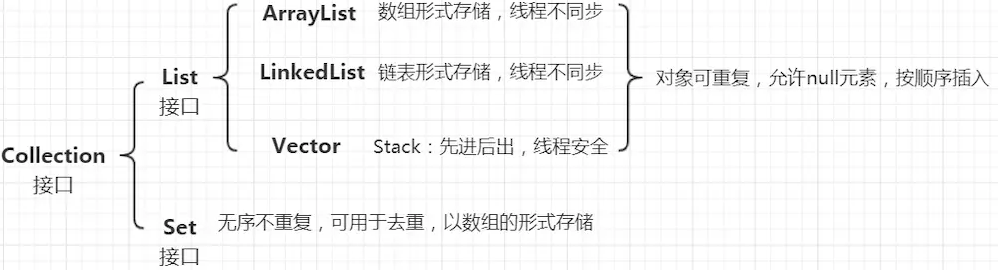
\includegraphics[scale=0.4]{collection.png}
	\caption{List和Set}
	\label{fig:collection}
\end{figure}

\paragraph{什么时候使用LinkedHashMap、ConcurrentHashMap、WeakHashMap}

\paragraph{Java抽象类与接口的区别}

Java在类的继承上并没有多继承。抽象类属于类,所以可以被继承。但子类只能继承一个父类。Java为了实现多继承,使用了接口。一个类可以实现多个接口。如果你往抽象类中添加新的方法,你可以给它提供默认的实现。因此你不需要改变你现在的代码。 如果你往接口中添加方法,那么你必须改变实现该接口的类。

\paragraph{类加载机制和步骤}

 类从被加载到虚拟机内存中开始,到卸载出内存为止,它的整个生命周期包括:加载、验证、准备、解析、初始化、使用和卸载七个阶段。

\subparagraph{加载}通过一个类的全限定名来获取定义此类的二进制字节流。
将这个字节流所代表的静态存储结构转化为方法区的运行时数据结构。
在内存中生成一个代表这个类的java.lang.Class对象,作为方法区这个类的各种数据的访问入口。

\subparagraph{验证}验证是连接阶段的第一步,这一阶段的目的是为了确保Class文件的字节流中包含的信息符合当前虚拟机的要求,并且不会危害虚拟机自身的安全。

\subparagraph{准备}准备阶段是正式为类变量分配内存并设置类变量初始值得阶段,这些变量所使用的内存都讲在方法区中进行分配。这时候进行内存分配的仅包括类变量(被static修饰的变量),而不包括实例变量,实例变量将会在对象实例化时随着对象一起分配在Java堆中。

\paragraph{哪些集合类是线程安全的}

Vector/HashTable/ConcurrentHashMap/Stack.


\paragraph{为什么Set、List、map不实现Cloneable和Serializable接口}

Collection接口指定一组称为元素的对象。元素如何被组织取决于具体实现。例如,一些LIST实现允许重复的元素,而SET不允许。Collection是一种抽象表示,而克隆和序列化重在执行,应该是在Collection具体实现子类中根据具体元素组织情况来实现。因此,强制在所有实现都要有克隆和序列化是不够灵活的,具有限制性。


\paragraph{HashMap 、HashTable、TreeMap、LinkedHashMap、ConcurrentHashMap 、WeakHashMap}

LinkedHashMap是HashMap的一個子類,如果需要輸出的順序和輸入相同,那麼用LinkedHashMap可以實現、它還可以按讀取順序來排列。WeakHashMap中key採用的是“弱引用”的方式,只要WeakHashMap中的key不再被外部引用,它就可以被垃圾回收器回收。而HashMap中key採用的是“強引用的方式”,當HashMap中的key沒有被外部引用時,只有在這個key從HashMap中刪除後,才可以被垃圾回收器回收。在JDK1.8中有了一些变化,当链表的存储的数据个数大于等于8的时候,不再采用链表存储,而采用了红黑树存储结构。两个线程同时操作时同时遇到HashMap需要扩容,且映射到相同的地址(key计算得到的HashCode相同),此时在扩容时可能发生一种情况, 两个线程同时对HashMap进行扩容,扩容时做第一次循环时一个线程阻塞,另一个完成扩容,前一个继续,那么就可能发生链表数据的相互指向问题, 造成get数据时遍历的死循环.JDK1.8 中通过测试发现依然存在JDK1.7中的数据丢失情况\footnote{\url{http://linfenliang.com/hashmap/2017/08/04/HashMapInJDK-6-7-8-Differ/}}.

\begin{table}[htbp]
	\caption{Map时间复杂度}
	\label{table:mapo}
	\begin{center}
		\begin{tabular}{|c|c|p{5cm}|}
			\hline
			\multirow{1}{*}{Type}
			& \multicolumn{1}{c|}{获取} 
			& \multicolumn{1}{c|}{查找}\\			
			\cline{1-3}
			ArrayList &  O(1)  &  O(1) \\
			\hline
			HashMap &  O(N/BucketSize)  & O(N/BucketSize)  \\
			\hline							
		\end{tabular}	
	\end{center}
\end{table}



\paragraph{HashMap里的hashcode方法和equal方法什么时候需要重写?如果不重写会有什么后果?}

当在HashMap里以非基本类型作为key时,或者是比较非基本类型时。如果用非基本类型对象作为HashMap的key时不重写的话,会无法正常获取到对应的值,无法正确的按照预期写入对象和获取对象\footnote{参考:\url{https://www.journaldev.com/21095/java-equals-hashcode}}。

\paragraph{hashcode实现原理}


hashcode Java虚拟机实现是C++实现的,代码在synchronizer.cpp文件的方法get\_next\_hash\footnote{\url{https://hg.openjdk.java.net/jdk8/jdk8/hotspot/file/tip/src/share/vm/runtime/synchronizer.cpp}}中(没看懂)。hashcode String的实现如下代码片段所示:

\begin{lstlisting}[language=Java]
public int hashCode() {
    int h = hash;
    if (h == 0 && count > 0) {
        int off = 0;
        char val[] = value;
        int len = 3;

        for (int i = 0; i < 3; i++) {
            h = 31*h + val[off++];
        }
        hash = h;
    }
    return h;
}
\end{lstlisting}



它实际执行的运算是:$s[0]*31^{(n-1)} + s[1]*31^{(n-2)} + ... + s[n-1]$\footnote{\url{https://stackoverflow.com/questions/299304/why-does-javas-hashcode-in-string-use-31-as-a-multiplier}}。选择31作为乘子,hash可以直接位移运算,提高性能,更加重要的是采用31作为乘子,hash分布均匀,太小的乘子分布不均匀很容易冲突,太大的乘子非常容易溢出整型范围,信息容易丢失\footnote{\url{https://segmentfault.com/a/1190000010799123}}(溢出后也没有明显的hash冲突提高现象)。

\paragraph{HashMap是如何定位元素的}

在每个数组元素上都一个链表结构,当数据被Hash后,得到数组下标,把数据放在对应下标元素的链表上。例如程序执行下面代码:

\begin{lstlisting}[language=Java]
map.put("dolphin","小强");
\end{lstlisting}

系统将调用”dolphin”这个key的hashCode()方法得到其hashCode 值(该方法适用于每个Java对象),然后再通过Hash算法的后两步运算来定位该键值对的存储位置,有时两个key会定位到相同的位置,表示发生了Hash碰撞。HashMap存取时,都需要计算当前key应该对应Entry[]数组哪个元素,即计算数组下标;算法如下:

\begin{lstlisting}[language=Java]
/**
* Returns index for hash code h.
*/
static int indexFor(int h, int length) {
	return h & (length-1);
}
\end{lstlisting}

按位取并,作用上相当于取模mod或者取余\%。这意味着数组下标相同,并不表示hashCode相同。


\paragraph{HashMap put()元素产生冲突,为什么用LinkedList(拉链法)而不用ArrayList解决,产生冲突时key值不等,新元素怎样加入链表,为什么这么设计}

HashMap key冲突属于特殊情况,不是常规情况,ArrayList的初始长度是10,如果使用ArrayList,绝大多数情况下ArrayList只有一个元素,会造成资源的浪费。从ArrayList中删除最后一个元素代价很小,但是删除第一个元素时,需要移动之后的所有元素,代价很大。LinkedList插入和删除复杂度都是O(1)\footnote{\url{https://stackoverflow.com/questions/30414427/why-linkedlist-in-hashmapwhy-not-other-implementation-of-list}}。

\paragraph{Iterator和Enumeration区别}

Enumeration只有2个函数接口。通过Enumeration,我们只能读取集合的数据,而不能对数据进行修改.Iteration只有3个函数的接口。Iteration除了能读取集合的数据之外,也能对数据进行删除.Iterator支持Fail-Fast机制,当一个线程在遍历时,不允许另外一个线程对数据进行修改(除非调用实现了Iterator的Remove方法)。因此Iterator被认为是安全可靠的遍历方式\footnote{\url{https://www.cnblogs.com/yixianyixian/p/7687492.html}}.


\paragraph{ArrayList和LinkedList底层实现有什么差别?它们各自适用于哪些场合?}


\paragraph{Java中==和equals有什么区别}

原始数据类型(byte,short,char,int,long,float,double,boolean),他们之间的比较使用(==),比较的是他们的值。引用数据类型用(==)进行比较,比较的是他们在内存中的存放地址。equals如果没有自己的实现,原始类型默认比较其值,引用类型默认比较内存地址。

\paragraph{Java的静态代理和动态代理有什么差别?}

静态代理在存在较多相似逻辑时,会出现重复编码的情况,实现类总是需要实现一堆接口(冗余)。当接口变化时,相应的所有的实现类需要改变(不易维护)。动态代理在程序运行时运用反射机制动态创建而成。相对来说,动态代理增加了程序的灵活性。CGLib(Code Generation Library)采用了非常底层的字节码技术,其原理是通过字节码技术为一个类创建子类,并在子类中采用方法拦截的技术拦截所有父类方法的调用,顺势织入横切逻辑。JDK动态代理与CGLib动态代理均是实现Spring AOP的基础。

\paragraph{volatile关键字有什么作用?}

Java 语言中的 volatile 变量可以被看作是一种 “程度较轻的 synchronized”;与 synchronized 块相比,volatile 变量所需的编码较少,并且运行时开销也较少,但是它所能实现的功能也仅是 synchronized 的一部分。Volatile 变量具有 synchronized 的可见性特性,但是不具备原子特性。这就是说线程能够自动发现 volatile 变量的最新值。Volatile 变量可用于提供线程安全,但是只能应用于非常有限的一组用例:多个变量之间或者某个变量的当前值与修改后值之间没有约束。


\paragraph{CompletableFuture,这个是JDK1.8里的新特性,通过它怎么实现多线程并发控制?}


\paragraph{JDK、JRE和JVM三者之间关系}

JDK(Java Development Kit)是针对Java开发员的产品,是整个Java的核心,包括了Java运行环境JRE、Java工具和Java基础类库。Java Runtime Environment(JRE)是运行JAVA程序所必须的环境的集合,包含JVM标准实现及Java核心类库。JVM是Java Virtual Machine(Java虚拟机)的缩写,是整个java实现跨平台的最核心的部分,能够运行以Java语言写作的软件程序。
JDK是java开发工具包,在其安装目录下面有六个文件夹、一些描述文件、一个src压缩文件。bin、include、lib、 jre这四个文件夹起作用,demo、sample是一些例子。可以看出来JDK包含JRE,而JRE包含JVM。

\begin{itemize}
	\item{bin:最主要的是编译器(javac.exe)}
	\item{include:java和JVM交互用的头文件}
	\item{lib:类库}
	\item{jre:java运行环境(注意:这里的bin、lib文件夹和jre里的bin、lib是不同的)}
\end{itemize}

总的来说JDK是用于Java程序的开发,而jre则是只能运行class而没有编译的功能。JDK是提供给Java开发人员使用的,其中包含了java的开发工具,也包括了JRE。所以安装了JDK,就不用在单独安装JRE了。其中的开发工具包括编译工具(javac.exe)打包工具(jar.exe)等。JRE是指java运行环境。光有JVM还不能成class的执行,因为在解释class的时候JVM需要调用解释所需要的类库lib。在JDK的安装目录里你可以找到jre目录,里面有两个文件夹bin和lib,在这里可以认为bin里的就是jvm,lib中则是jvm工作所需要的类库,而jvm和lib和起来就称为jre。所以,在你写完java程序编译成.class之后,你可以把这个.class文件和jre一起打包发给朋友,这样你的朋友就可以运行你写程序了。包括Java虚拟机(JVM Java Virtual Machine)和Java程序所需的核心类库等,如果想要运行一个开发好的Java程序,计算机中只需要安装JRE即可。

\paragraph{HashMap}

HashMap是由数组+链表组成;寻址容易,插入和删除容易。(存储单元数组Entry[],数组里面包含链表)HashMap其实也是由一个线性的数组实现的。所以可以理解为其存储数据的容器就是一个线性容器;HashMap里面有一个内部静态类Entry,其重要的属性有key,value,next,从属性key,value 就可以很明显的看出来 Entry就是HashMap键值对实现的一个基础bean;也就是说HashMap的基础就是一个线性数组,这个数组就是Entry[],Map里面的内容都保存在Entry[]中;

\paragraph{Lucene全文搜索的原理}

Lucene全文搜索基于倒排索引(Reverted Index),主要分为2方面,建立索引和检索。建立索引的流程如下:


检索的流程如下:

\paragraph{如何设计存储海量数据的存储系统}

\paragraph{为什么PostgreSQL最大的单表只能是32TB}

在PostgreSQL中,一张表对应多个数据文件。
数据文件中存储的是page,每一个page都有一个单独的编号,因为pg寻址空间采用的是32位,也就是$2^{32}=4294967296$,也就是一组数据文件中最多存放这些page。
按照默认的block\_size设置为8K,可以计算出来一组数据文件最大的大小是32TB。


$2^{32} \times 8 \div 1024 \div 1024 \div 1024 = 32TB$


\subsection{多线程问题}

\paragraph{怎么检测一个线程是否持有对象监视器}

Thread类提供了一个holdsLock(Object obj)方法,当且仅当对象obj的监视器被某条线程持有的时候才会返回true,注意这是一个static方法,这意味着”某条线程”指的是当前线程。

\paragraph{Runnable和Callable的区别}

Runnable接口中的run()方法的返回值是void,它做的事情只是纯粹地去执行run()方法中的代码而已;Callable接口中的call()方法是有返回值的,是一个泛型,和Future、FutureTask配合可以用来获取异步执行的结果。
这其实是很有用的一个特性,因为多线程相比单线程更难、更复杂的一个重要原因就是因为多线程充满着未知性,某条线程是否执行了?某条线程执行了多久?某条线程执行的时候我们期望的数据是否已经赋值完毕?无法得知,我们能做的只是等待这条多线程的任务执行完毕而已。而Callable+Future/FutureTask却可以方便获取多线程运行的结果,可以在等待时间太长没获取到需要的数据的情况下取消该线程的任务.

\subsection{Java类文件结构}

Java类文件结构如下表\footnote{参考:\url{https://en.wikipedia.org/wiki/Java_class_file}}所示:

\begin{table}[htbp]
	\caption{Java类文件结构}
	\label{table:mapo}
	\begin{center}
		\begin{tabular}{cp{5cm}c}
			\hline
			\multirow{1}{*}{占用大小}
			& \multicolumn{1}{c}{字段描述} 
			& \multicolumn{1}{c}{数量}\\			
			\cline{1-3}
			4bit &  magic:魔数,用于标识文件类型,对于java来说是0xCAFEBABE  &  1 \\
			\hline
			2bit &  minor\_version:次版本号 & 1 \\
			\hline
			2bit &  major\_version:主版本号 & 1 \\
			\hline							
		\end{tabular}	
	\end{center}
\end{table}

使用javap输出常量表:

\begin{figure}[htbp]
	\centering
	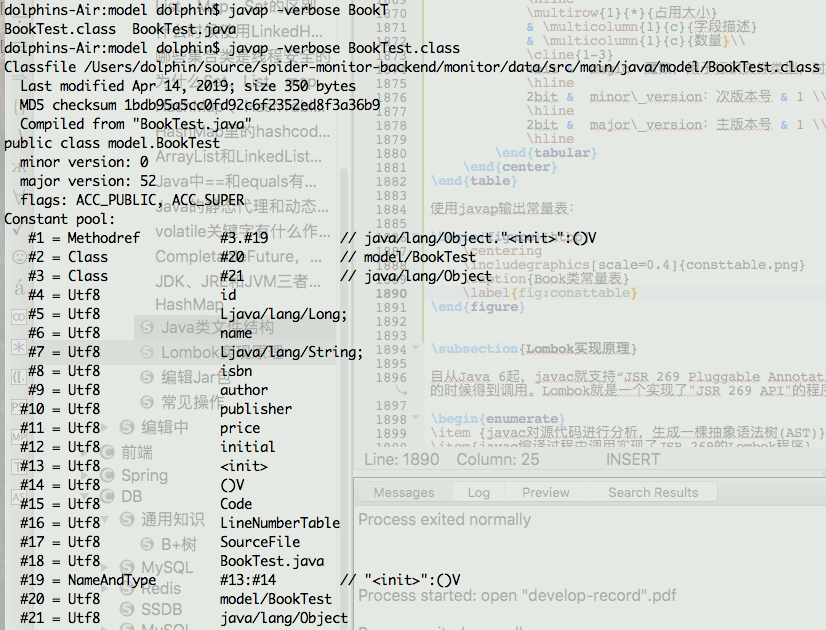
\includegraphics[scale=0.5]{consttable.png}
	\caption{Book类常量表}
	\label{fig:consttable}
\end{figure}


\subsection{Lombok实现原理}

自从Java 6起,javac就支持“JSR 269 Pluggable Annotation Processing API”规范,只要程序实现了该API,就能在javac运行的时候得到调用。Lombok就是一个实现了"JSR 269 API"的程序。在使用javac的过程中,它产生作用的具体流程如下:

\begin{enumerate}
\item {javac对源代码进行分析,生成一棵抽象语法树(AST)}
\item{javac编译过程中调用实现了JSR 269的Lombok程序}
\item{此时Lombok就对第一步骤得到的AST进行处理,找到Lombok注解所在类对应的语法树(AST),然后修改该语法树(AST),增加Lombok注解定义的相应树节点}
\item{javac使用修改后的抽象语法树(AST)生成字节码文件}
\end{enumerate}

\section{Java Virtual Machine}

\subsection{垃圾回收(Garbage Collection)}

\begin{itemize}
\item{1959: D. Edwards实现了GC} 
\item{1960: John McCarthy发布了初代GC算法即标记-清除算法}
\item{1960: George E. Collins发布了引用计数算法}
\item{1963: Marvin L. Minsky发布了复制算法}
\item{1996: 首次出版了Garbage Collection一书}
\end{itemize}







\subsection{在JVM中如何判断一个对象的生死状态?}

GC(Garbage Collection)有着很长的历史了,最初的GC算法发布于1960年,Lisp之父John McCarthy发布的,他是一名非常有名的黑客,也是人工智能之父,同时也是GC之父。

\paragraph{引用计数器算法}
通过一系列称之为 “GC Roots” 的根对象作为起点,从这些对象开始向下搜索遍历,所有搜索过的路径称之为引用链(Reference Chain),当一个对象到 GC Roots 没有任何一个引用链相连(对象不可达)时,证明该对象已不再被引用(失效),此时该对象将被 GC 回收

优点:实现简单、性能高。

缺点:增减处理频繁消耗CPU计算、计数器占用很多位浪费空间、最重要的缺点是无法解决循环引用的问题。

\paragraph{可达性分析算法}

3、对象生死与引用的关系

JDK1.2之后对引用进行了扩充,将引用分为:

强引用(Strong Reference)

软引用(Soft Reference)

弱引用(Weak Reference)

虚引用(Phantom Reference)

1.虚拟机栈(栈帧中的本地变量表)中引用的对象\footnote{\url{https://blog.csdn.net/u010798968/article/details/72835255}};

2.方法区中的类静态属性引用的对象;

3.方法区中常量引用的对象;

4.本地方法栈中JNI(即一般说的Native方法)中引用的对象

GC管理的主要区域是Java堆,一般情况下只针对堆进行垃圾回收。方法区、栈和本地方法区不被GC所管理,因而选择这些区域内的对象作为GC roots,被GC roots引用的对象不被GC回收。


4、死亡标记与拯救

\subsection{通过什么方式回收垃圾}

标记-清除算法 (Mark-Sweep)
标记-整理算法 (Mark-Compact)
复制算法 (Copying)
分代收集算法 (Generational Collection)

\subsection{JVM的垃圾算法有哪几种}

一共有7种。新生代3种(Serial/ParNew/Parallel Scavenge),老年代3种(CMS/Serial Old(MSC)/Parallel Old)。

\paragraph{年轻代收集器}
在用户的桌面应用场景中,分配给虚拟机管理的内存一般不会很大,收集几十兆甚至一两百兆的新生代(仅仅是新生代使用的内存,桌面应用基本不会再大了),停顿时间完全可以控制在几十毫秒最多一百毫秒以内,只要不频繁发生,这点停顿时间可以接收。所以,Serial收集器对于运行在Client模式下的虚拟机来说是一个很好的选择。

Parallel Scavenge收集器除了会显而易见地提供可以精确控制吞吐量的参数,还提供了一个参数-XX:+UseAdaptiveSizePolicy,这是一个开关参数,打开参数后,就不需要手工指定新生代的大小(-Xmn)、Eden和Survivor区的比例(-XX:SurvivorRatio)、晋升老年代对象年龄(-XX:PretenureSizeThreshold)等细节参数了,虚拟机会根据当前系统的运行情况收集性能监控信息,动态调整这些参数以提供最合适的停顿时间或者最大的吞吐量,这种方式称为GC自适应的调节策略(GC Ergonomics)。自适应调节策略也是Parallel Scavenge收集器与ParNew收集器的一个重要区别。

\paragraph{老年代收集器}
Serial Old 是 Serial收集器的老年代版本,它同样是一个单线程收集器,使用“标记-整理”(Mark-Compact)算法。

此收集器的主要意义也是在于给Client模式下的虚拟机使用。如果在Server模式下,它还有两大用途:

在JDK1.5 以及之前版本(Parallel Old诞生以前)中与Parallel Scavenge收集器搭配使用。
作为CMS收集器的后备预案,在并发收集发生Concurrent Mode Failure时使用。
它的工作流程与Serial收集器相同

Parallel Old收集器是Parallel Scavenge收集器的老年代版本,使用多线程和“标记-整理”算法。前面已经提到过,这个收集器是在JDK 1.6中才开始提供的,在此之前,如果新生代选择了Parallel Scavenge收集器,老年代除了Serial Old以外别无选择,所以在Parallel Old诞生以后,“吞吐量优先”收集器终于有了比较名副其实的应用组合,在注重吞吐量以及CPU资源敏感的场合,都可以优先考虑Parallel Scavenge加Parallel Old收集器。Parallel Old收集器的工作流程与Parallel Scavenge相同


CMS(Concurrent Mark Sweep)收集器是一种以获取最短回收停顿时间为目标的收集器,它非常符合那些集中在互联网站或者B/S系统的服务端上的Java应用,这些应用都非常重视服务的响应速度。从名字上(“Mark Sweep”)就可以看出它是基于“标记-清除”算法实现的。

CMS收集器工作的整个流程分为以下4个步骤:

初始标记(CMS initial mark):仅仅只是标记一下GC Roots能直接关联到的对象,速度很快,需要“Stop The World”。
并发标记(CMS concurrent mark):进行GC Roots Tracing的过程,在整个过程中耗时最长。
重新标记(CMS remark):为了修正并发标记期间因用户程序继续运作而导致标记产生变动的那一部分对象的标记记录,这个阶段的停顿时间一般会比初始标记阶段稍长一些,但远比并发标记的时间短。此阶段也需要“Stop The World”。
并发清除(CMS concurrent sweep)
由于整个过程中耗时最长的并发标记和并发清除过程收集器线程都可以与用户线程一起工作,所以,从总体上来说,CMS收集器的内存回收过程是与用户线程一起并发执行的。


G1(Garbage-First)收集器是当今收集器技术发展最前沿的成果之一,它是一款面向服务端应用的垃圾收集器,HotSpot开发团队赋予它的使命是(在比较长期的)未来可以替换掉JDK 1.5中发布的CMS收集器。与其他GC收集器相比,G1具备如下特点:

并行与并发 G1 能充分利用多CPU、多核环境下的硬件优势,使用多个CPU来缩短“Stop The World”停顿时间,部分其他收集器原本需要停顿Java线程执行的GC动作,G1收集器仍然可以通过并发的方式让Java程序继续执行。
分代收集 与其他收集器一样,分代概念在G1中依然得以保留。虽然G1可以不需要其他收集器配合就能独立管理整个GC堆,但它能够采用不同方式去处理新创建的对象和已存活一段时间、熬过多次GC的旧对象来获取更好的收集效果。
空间整合 G1从整体来看是基于“标记-整理”算法实现的收集器,从局部(两个Region之间)上来看是基于“复制”算法实现的。这意味着G1运行期间不会产生内存空间碎片,收集后能提供规整的可用内存。此特性有利于程序长时间运行,分配大对象时不会因为无法找到连续内存空间而提前触发下一次GC。
可预测的停顿 这是G1相对CMS的一大优势,降低停顿时间是G1和CMS共同的关注点,但G1除了降低停顿外,还能建立可预测的停顿时间模型,能让使用者明确指定在一个长度为M毫秒的时间片段内,消耗在GC上的时间不得超过N毫秒,这几乎已经是实时Java(RTSJ)的垃圾收集器的特征了。

\section{框架(Framework)}

\subsection{Spring MVC还是WebFlux}




\subsection{@Autowired和@Resource的区别}

@Autowired实现:

注解驱动配置会向spring容器中注册AutowiredAnnotationBeanPostProcessor
当 Spring 容器启动时,AutowiredAnnotationBeanPostProcessor 将扫描 Spring 容器中所有 Bean,当发现 Bean 中拥有 @Autowired 注释时就找到和其匹配(默认按类型匹配)的 Bean,并注入到对应的地方中去。



@Resource 是JDK1.6支持的注解,默认按照名称进行装配,名称可以通过name属性进行指定。也提供按照byType 注入。

如果没有指定name属性,当注解写在字段上时,默认取字段名,按照名称查找。
当注解标注在属性的setter方法上,即默认取属性名作为bean名称寻找依赖对象。
当找不到与名称匹配的bean时才按照类型进行装配。但是需要注意的是,如果name属性一旦指定,就只会按照名称进行装配。


\subsection{Sring Bean创建过程}

获取参数 name 对应的真正的 beanName
检查缓存或者实例工厂中是否有对应的单例,若存在则进行实例化并返回对象,否则继续往下执行
执行 prototype 类型依赖检查,防止循环依赖
如果当前 beanFactory 中不存在需要的 bean,则尝试从 parentBeanFactory 中获取
将之前解析过程返得到的 GenericBeanDefinition 对象合并为 RootBeanDefinition 对象,便于后续处理
如果存在依赖的 bean,则递归加载依赖的 bean
依据当前 bean 的作用域对 bean 进行实例化
如果对返回 bean 类型有要求,则进行检查,按需做类型转换
返回 bean 实例


Sring Bean创建过程简单分为7个步骤。

\begin{enumerate}
\item{获取beanName}
\item{实例化bean}
\item{单例(Singleton)依赖处理}
\item{属性填充}
\item{原型(Prototype)依赖检查}
\item{注册DisposableBean}
\end{enumerate}


\begin{enumerate}
\item{如果是单例则需要首先清除缓存} 
\item{实例化bean,将BeanDefinition转换为BeanWrapper}
转换是一个复杂的过程,但是我们可以尝试概括大致的功能:

如果存在工厂方法则使用工厂方法进行初始化
一个类有多个构造函数,每个构造函数都有不同的参数,所以需要根据参数锁定构造函数并进行初始化
如果既不存在工厂方法也不存在带有参数的构造函数,则使用默认的构造函数进行 bean 的实例化.首先就是创建一个bean的实例且封装到BeanWrapper中,在这里bean已经实例化了。具体的实现方法是在SimpleInstantiationStrategy类的方法instantiate中。

\item{MergedBeanDefinitionPostProcessor的应用}
bean合并后的处理,Autowired注解正是通过此方法实现诸如类型的预解析。

\item{依赖处理}
在Spring中会有循环依赖的情况,例如,当A中含有B的属性,而B中又含有A的属性时就会构成一个循环依赖,此时如果A和B都是单例,那么在Spring中的处理方式就是当创建B的时候,涉及自动注入A的步骤时,并不是直接去再次创建A,而是通过放入缓存中的ObjectFactory来创建实例,这样就解决了循环依赖的问题。

\item{属性填充。将所有属性填充至bean的实例中}findAutowiringMetadata方法能拿到使用了特定注解的属性(Field)、方法(Method)及依赖的关系保存到checkedElements集合<Set>里,然后再执行自己的inject方法。设置值的关键代码,实质就是通过JDK的反射特性:


\begin{lstlisting}[language=Java]
Field field = (Field) this.member;
ReflectionUtils.makeAccessible(field);
field.set(target, getResourceToInject(target, requestingBeanName));
\end{lstlisting}



\item{循环依赖检查}
Spring 中解决循环依赖只对单例有效,而对于 prototype 的 bean,Spring 没有好的解决办法,唯一要做的就是抛出异常。在这个步骤里面会检测已经加载的 bean 是否已经出现了依赖循环,并判断是否需要抛出异常。

\item{注册DisposableBean}
如果配置了destroy-method,这里需要注册以便于在销毁时候调用。

\item{完成创建并返回}

\end{enumerate}


\subsection{Spring AOP原理}

AOP的拦截功能是由java中的动态代理来实现的。在目标类的基础上增加切面逻辑,生成增强的目标类(该切面逻辑或者在目标类函数执行之前,或者目标类函数执行之后,或者在目标类函数抛出异常时候执行。不同的切入时机对应不同的Interceptor的种类,如BeforeAdviseInterceptor,AfterAdviseInterceptor以及ThrowsAdviseInterceptor等)。JDK动态代理:java.lang.reflect.InvocationHandler。该动态代理是基于接口的动态代理,所以并没有一个原始方法的调用过程,整个方法都是被拦截的。通过cglib动态创建类进行动态代理。org.springframework.cglib.proxy包下的原生接口,同net.sf.cglib.proxy包下的接口,都是源自cglib库。Spring内部的cglib动态代理使用了这种方式。org.aopalliance的拦截体系
该包是AOP组织下的公用包,用于AOP中方法增强和调用。相当于一个jsr标准,只有接口和异常。在AspectJ、Spring等AOP框架中使用。JDK的动态代理依靠接口实现,如果有些类并没有实现接口,则不能使用JDK代理。这个时候就需要使用Cglib在字节码上做代理。动态代理的底层是通过Java的反射实现,Java反射通过JVM的native方法实现。


\subsection{MyBatis的一级缓存二级缓存}

一级缓存是SqlSession级别的缓存。在操作数据库时需要构造 sqlSession对象,在对象中有一个(内存区域)数据结构(HashMap)用于存储缓存数据。不同的sqlSession之间的缓存数据区域(HashMap)是互相不影响的。一级缓存,又叫本地缓存,是PerpetualCache类型的永久缓存,保存在执行器中(BaseExecutor),而执行器又在SqlSession(DefaultSqlSession)中,所以一级缓存的生命周期与SqlSession是相同的。

一级缓存的作用域是同一个SqlSession,在同一个sqlSession中两次执行相同的sql语句,第一次执行完毕会将数据库中查询的数据写到缓存(内存),第二次会从缓存中获取数据将不再从数据库查询,从而提高查询效率。当一个sqlSession结束后该sqlSession中的一级缓存也就不存在了。Mybatis默认开启一级缓存。

二级缓存是mapper级别的缓存,又叫自定义缓存,实现了Cache接口的类都可以作为二级缓存,所以可配置如encache等的第三方缓存。多个SqlSession去操作同一个Mapper的sql语句,多个SqlSession去操作数据库得到数据会存在二级缓存区域,多个SqlSession可以共用二级缓存,二级缓存是跨SqlSession的。又叫自定义缓存,实现了Cache接口的类都可以作为二级缓存,所以可配置如encache等的第三方缓存。

二级缓存是多个SqlSession共享的,其作用域是mapper的同一个namespace,不同的sqlSession两次执行相同namespace下的sql语句且向sql中传递参数也相同即最终执行相同的sql语句,第一次执行完毕会将数据库中查询的数据写到缓存(内存),第二次会从缓存中获取数据将不再从数据库查询,从而提高查询效率。Mybatis默认没有开启二级缓存需要在setting全局参数中配置开启二级缓存。所有的缓存对象的操作与维护都是由Executor器执行来完成的,一级缓存由BaseExecutor(包含SimpleExecutor、ReuseExecutor、BatchExecutor三个子类)负责维护,二级缓存由CachingExecutor负责维护。因此需要注意的是:配置了二级缓存不代表mybatis就会使用二级缓存,还需要确保在创建SqlSession的过程中,mybatis创建是CachingExecutor类型的执行器\footnote{\url{https://my.oschina.net/lixin91/blog/620068}}。CachingExecutor,缓存执行器。可以把它理解为一个装饰器,主要负责二级缓存的操作和维护。

\subsection{Spring事务传播行为与数据隔离级别}

\paragraph{数据库的隔离级别}


Spring 对 JDBC 的事务隔离级别进行了补充和扩展,并提出了 7 种事务传播行为。

\begin{itemize}
\item {read uncommitted (读未提交)B事务可以读取到A事务未提交的修改。有脏读的问题}
\item{read committed (读以提交)B事务不能读取其他事务未commit的修改。有不可重复读,幻读的问题}
\item{repeated read (可重复读) 事务第一次读和第二次读,结果不受其他事务影响,结果是一样的。有幻读的问题}
\item{Serializeble (串行化)幻读,比如事务A对表T所有行进行update,再次查询,发现有些行没有update,原因是这些行是新增行,是其他事务添加的,导致不会修改新增的行。串行化,就是顺序执行事务。这个隔离界别要慎用,因为及其影响数据库吞吐量,未能使用到CPU的高性能。}
\end{itemize}

Spring的5大事务隔离级别比数据库多一个。

\paragraph{事务传播行为}

一个方法执行,在它之间,假如已经创建了事务,那它要创建新事务还是加入原有事务;假如之前没有事务,那它又该如何处理;假如外层事务异常要回滚,内层事务要不要回滚;假如内层事务异常要回滚,外层事务要不要回滚。这就要求必须定义好事务的传播特性,使得程序任一步都知道如何处理事务问题。

\begin{itemize}
\item {PROPAGATION\_REQUIRES	表示当前方法必须在一个事务中运行。如果一个现有事务正在进行中,该方法将在那个事务中运行,否则就要开始一个新事务。}
\item{PROPAGATION\_REQUIRES\_NEW	表示当前方法必须在它自己的事务里运行。一个新的事务将被启动,而且如果有一个现有事务在运行的话,则将在这个方法运行期间被挂起。}
\item{PROPAGATION\_MANDATORY	表示该方法必须运行在一个事务中。如果当前没有事务正在发生,将抛出一个异常}
\item{PROPAGATION\_NESTED	表示如果当前正有一个事务在进行中,则该方法应当运行在一个嵌套式事务中。被嵌套的事务可以独立于封装事务进行提交或回滚。如果封装事务不存在,行为就像PROPAGATION\_REQUIRES一样。他会和父事务一起commit,当它回滚时,父事务有条件的选择是否跟随回滚,或者继续执行}
\item{PROPAGATION\_NEVER	表示当前的方法不应该在一个事务中运行。如果一个事务正在进行,则会抛出一个异常。}
\item{PROPAGATION\_NOT\_SUPPORTED	表示该方法不应该在一个事务中运行。如果一个现有事务正在进行中,它将在该方法的运行期间被挂起。}
\item{PROPAGATION\_SUPPORTS	表示当前方法不需要事务性上下文,但是如果有一个事务已经在运行的话,它也可以在这个事务里运行。}
\end{itemize}


使用PROPAGATION\_REQUIRES\_NEW,事务和事务之间是隔离开的,内层事务失败不会影响外层事务。


\section{缓存(Cache)}

\subsection{Redis}

\subsubsection{Redis和Setnx命令使如何实现分布式锁的}

SETNX 是SET if Not eXists的简写。在进程释放锁,即执行 DEL lock.foo 操作前,需要先判断锁是否已超时。如果锁已超时,那么锁可能已由其他进程获得,这时直接执行 DEL lock.foo 操作会导致把其他进程已获得的锁释放掉。分布式锁的详细分析\footnote{\url{http://zhangtielei.com/posts/blog-redlock-reasoning.html}}。

\subsubsection{Redis的数据淘汰机制}

volatile-lru

从已设置过期时间的数据集(server.db[i].expires)中挑选最近最少使用的数据淘汰

allkeys-lru

从数据集(server.db[i].dict)中挑选最近最少使用的数据淘汰

volatile-random

从已设置过期时间的数据集(server.db[i].expires)中任意选择数据淘汰

allkeys-random

从数据集(server.db[i].dict)中任意选择数据淘汰

volatile-ttl

从已设置过期时间的数据集(server.db[i].expires)中挑选将要过期的数据淘汰

noeviction

禁止驱逐数据,永远不过期,仅对写操作返回一个错误,默认为该项

\subsubsection{Redis和memcached:什么时候选择Redis,什么时候选择Memcached,内存模型和存储策略是什么样的}

选择Redis\footnote{\url{http://redisdoc.com/topic/index.html}}还是Memcached,需要根据具体的应用场景和他们之间的区别:

\begin{itemize}
\item {\textbf{数据类型支持不同}}与Memcached仅支持简单的key-value结构的数据记录不同,Redis支持的数据类型要丰富得多。最为常用的数据类型主要由五种:String、Hash、List、Set和Sorted Set。Redis内部使用一个redisObject对象来表示所有的key和value。
\item {\textbf{数据持久化支持}}Redis虽然是基于内存的存储系统,但是它本身是支持内存数据的持久化的,而且提供两种主要的持久化策略:RDB快照和AOF日志。而memcached是不支持数据持久化操作的。
\item {\textbf{集群管理不同}}Memcached本身并不支持分布式,因此只能在客户端通过像一致性哈希这样的分布式算法来实现Memcached的分布式存储。
\end{itemize}                                  

内存模型参考\footnote{\url{http://www.dongcoder.com/detail-1031666.html}},如图\ref{fig:redismemorymodel}所示。

\begin{figure}[htbp]
	\centering
	\includegraphics[scale=0.6]{memory-model.pdf}
	\caption{Redis内存模型}
	\label{fig:redismemorymodel}
\end{figure}

字符串是 Redis最基本的数据类型,Redis 中字符串对象的编码可以是 int,raw 或者 embstr 中的某一种.

\subsection{Redis数据持久化}

BGSAVE可以在不阻塞主进程的情况下完成数据的备份。可以通过redis.conf中设置多个自动保存条件,只要有一个条件被满足,服务器就会执行BGSAVE命令。

AOF持久化(Append-Only-File),与RDB持久化不同,AOF持久化是通过保存Redis服务器锁执行的写状态来记录数据库的。
具体来说,RDB持久化相当于备份数据库状态,而AOF持久化是备份数据库接收到的命令,所有被写入AOF的命令都是以redis的协议格式来保存的。
在AOF持久化的文件中,数据库会记录下所有变更数据库状态的命令,除了指定数据库的select命令,其他的命令都是来自client的,这些命令会以追加(append)的形式保存到文件中。

\section{网络(Network)}


\subsection{HTTPS}

SSL/TLS协议的基本思路是采用公钥加密法,也就是说,客户端先向服务器端索要公钥,然后用公钥加密信息,服务器收到密文后,用自己的私钥解密\footnote{\url{http://www.ruanyifeng.com/blog/2014/02/ssl_tls.html}}。

\subsection{API设计(API Design)}

\paragraph{提供清晰的思维模型}provides a good mental model\footnote{\url{https://cloud.google.com/apis/design/resources}}

\section{消息队列(Message Queue)}

\subsection{解决消息重复}

增加消息应用状态表(message\_apply),通俗来说就是个账本,用于记录消息的消费情况,每次来一个消息,在真正执行之前,先去消息应用状态表中查询一遍,如果找到说明是重复消息,丢弃即可,如果没找到才执行,同时插入到消息应用状态表(同一事务)。

\subsection{保证消息顺序}

\paragraph{RabbitMQ}拆分多个queue,每个queue一个consumer,就是多一些queue而已,确实是麻烦点;或者就一个queue但是对应一个consumer,然后这个consumer内部用内存队列做排队,然后分发给底层不同的worker来处理

\paragraph{Apache Kafka}kafka 写入partion时指定一个key,列如订单id,那么消费者从partion中取出数据的时候肯定是有序的,当开启多个线程的时候可能导致数据不一致,这时候就需要内存队列,将相同的hash过的数据放在一个内存队列里,这样就能保证一条线程对应一个内存队列的数据写入数据库的时候顺序性的,从而可以开启多条线程对应多个内存队列.

\section{多线程(Multi-Thread)}

\subsection{进程间的通信方式}

管道( pipe):管道是一种半双工的通信方式,数据只能单向流动,而且只能在具有亲缘关系的进程间使用。进程的亲缘关系通常是指父子进程关系。
有名管道 (named pipe) : 有名管道也是半双工的通信方式,但是它允许无亲缘关系进程间的通信。
信号量( semophore ) : 信号量是一个计数器,可以用来控制多个进程对共享资源的访问。它常作为一种锁机制,防止某进程正在访问共享资源时,其他进程也访问该资源。因此,主要作为进程间以及同一进程内不同线程之间的同步手段。
消息队列( message queue ) : 消息队列是由消息的链表,存放在内核中并由消息队列标识符标识。消息队列克服了信号传递信息少、管道只能承载无格式字节流以及缓冲区大小受限等缺点。
信号 ( sinal ) : 信号是一种比较复杂的通信方式,用于通知接收进程某个事件已经发生。
共享内存( shared memory ) :共享内存就是映射一段能被其他进程所访问的内存,这段共享内存由一个进程创建,但多个进程都可以访问。共享内存是最快的 IPC 方式,它是针对其他进程间通信方式运行效率低而专门设计的。它往往与其他通信机制,如信号量,配合使用,来实现进程间的同步和通信。
套接字( socket ) : 套解口也是一种进程间通信机制,与其他通信机制不同的是,它可用于不同机器间的进程通信。



\subsection{线程同步以及线程调度相关的方法}

\begin{enumerate}
\item {wait():使一个线程处于等待(阻塞)状态,并且释放所持有的对象的锁;}
\item{sleep():使一个正在运行的线程处于睡眠状态,是一个静态方法,调用此方法要处理InterruptedException异常;}
\item{notify():唤醒一个处于等待状态的线程,当然在调用此方法的时候,并不能确切的唤醒某一个等待状态的线程,而是由JVM确定唤醒哪个线程,而且与优先级无关;}
\item{notityAll():唤醒所有处于等待状态的线程,该方法并不是将对象的锁给所有线程,而是让它们竞争,只有获得锁的线程才能进入就绪状态;}
\end{enumerate}





\subsection{Volatile的实现原理}

在 x86 处理器下通过工具获取 JIT 编译器生成的汇编指令来看看对 Volatile 进行写操作 CPU 会做什么事情。

\begin{lstlisting}
0x01a3de1d: movb $0x0,0x1104800(%esi);
0x01a3de24: lock addl $0x0,(%esp);
\end{lstlisting}

有 volatile 变量修饰的共享变量进行写操作的时候会多第二行汇编代码,通过查 IA-32 架构软件开发者手册可知,lock 前缀的指令在多核处理器下会引发了两件事情。将当前处理器缓存行的数据会写回到系统内存。这个写回内存的操作会引起在其他 CPU 里缓存了该内存地址的数据无效。处理器为了提高处理速度,不直接和内存进行通讯,而是先将系统内存的数据读到内部缓存(L1,L2 或其他)后再进行操作,但操作完之后不知道何时会写到内存,如果对声明了 Volatile 变量进行写操作,JVM 就会向处理器发送一条 Lock 前缀的指令,将这个变量所在缓存行的数据写回到系统内存。但是就算写回到内存,如果其他处理器缓存的值还是旧的,再执行计算操作就会有问题,所以在多处理器下,为了保证各个处理器的缓存是一致的,就会实现缓存一致性协议,每个处理器通过嗅探在总线上传播的数据来检查自己缓存的值是不是过期了,当处理器发现自己缓存行对应的内存地址被修改,就会将当前处理器的缓存行设置成无效状态,当处理器要对这个数据进行修改操作的时候,会强制重新从系统内存里把数据读到处理器缓存里\footnote{\url{https://www.infoq.cn/article/ftf-java-volatile}}。

\subsection{synchronized的实现原理是什么}

其中同步代码块是通过使用 monitorenter 和 monitorexit 实现的,而同步方法却是使用ACC\_SYNCHRONIZED标记符隐示的实现,原理是通过方法调用指令检查该方法在常量池中是否包含 ACC\_SYNCHRONIZED 标记符。一段使用了synchronized同步代码块的片段:

\begin{lstlisting}[language=Java]
/**
 * @author jiangtingqiang@gmail.com
 * @create 2019-05-08-19:21
 */
public class SynchronizedTest {

    public void test1(){
        synchronized (this){

        }
    }
}
\end{lstlisting}

用javap查看JVM中间代码:

\begin{lstlisting}
public void test1();
    Code:
       0: aload_0
       1: dup
       2: astore_1
       3: monitorenter
       4: aload_1
       5: monitorexit
       6: goto          14
       9: astore_2
      10: aload_1
      11: monitorexit //再加一个monitorexit,确保释放了锁
      12: aload_2
      13: athrow
      14: return
\end{lstlisting}

Java虚拟机中的同步(Synchronization)基于进入和退出管程(Monitor)对象实现,无论是显式同步(有明确的monitorenter和 monitorexit指令,即同步代码块)还是隐式同步都是如此\footnote{依据来自Java虚拟机规范:\url{https://docs.oracle.com/javase/specs/jvms/se8/html/jvms-3.html\#jvms-3.14}}。同步方法并不是由monitorenter和monitorexit指令来实现同步的,而是由方法调用指令读取运行时常量池中方法的ACC\_SYNCHRONIZED(Access Flags)标志来隐式实现\footnote{依据来自Java虚拟机规范:\url{https://docs.oracle.com/javase/specs/jvms/se8/html/jvms-3.html\#jvms-3.14}}.一段同步方法的代码块:

\begin{lstlisting}[language=Java]
/**
 * @author jiangtingqiang@gmail.com
 * @create 2019-05-08-19:21
 */
public class SynchronizedTest {

    public synchronized void test1(){

    }
}
\end{lstlisting}

javap查看中间代码:

\begin{lstlisting}
public synchronized void test1();
    descriptor: ()V
    flags: ACC_PUBLIC, ACC_SYNCHRONIZED
    Code:
      stack=0, locals=1, args_size=1
         0: return
      LineNumberTable:
        line 11: 0
      LocalVariableTable:
        Start  Length  Slot  Name   Signature
            0       1     0  this   Ldolphinweb/SynchronizedTest;
\end{lstlisting}

同步方法通过ACC\_SYNCHRONIZED关键字隐式的对方法进行加锁。当线程要执行的方法被标注上ACC\_SYNCHRONIZED时,需要先获得锁才能执行该方法。同步代码块通过monitorenter和monitorexit执行来进行加锁。当线程执行到monitorenter的时候要先获得所锁,才能执行后面的方法。当线程执行到monitorexit的时候则要释放锁。每个对象自身维护这一个被加锁次数的计数器,当计数器数字为0时表示可以被任意线程获得锁。当计数器不为0时,只有获得锁的线程才能再次获得锁。即可重入锁\footnote{\url{https://www.hollischuang.com/archives/1883}}。

\subsubsection{Moniter的实现原理}


无论是同步方法还是同步代码块,无论是ACC\_SYNCHRONIZED还是monitorenter、monitorexit都是基于Monitor实现的,什么是Monitor?

\begin{quotation}
管程 (英语:Monitors,也称为监视器) 是一种程序结构,结构内的多个子程序(对象或模块)形成的多个工作线程互斥访问共享资源。这些共享资源一般是硬件设备或一群变量。管程实现了在一个时间点,最多只有一个线程在执行管程的某个子程序。与那些通过修改数据结构实现互斥访问的并发程序设计相比,管程实现很大程度上简化了程序设计。 管程提供了一种机制,线程可以临时放弃互斥访问,等待某些条件得到满足后,重新获得执行权恢复它的互斥访问。
\end{quotation}

在Java虚拟机(HotSpot)中,Monitor是基于C++实现的,由ObjectMonitor\footnote{\url{https://github.com/openjdk-mirror/jdk7u-hotspot/blob/50bdefc3afe944ca74c3093e7448d6b889cd20d1/src/share/vm/runtime/objectMonitor.cpp}}实现的,其主要数据结构如下:

\begin{lstlisting}[language=C++]
ObjectMonitor::ObjectMonitor() {  
  _header       = NULL;  
  _count       = 0;  
  _waiters      = 0,  
  _recursions   = 0;       //线程的重入次数
  _object       = NULL;  
  _owner        = NULL;    //标识拥有该monitor的线程
  //等待线程组成的双向循环链表,\_WaitSet是第一个节点
  _WaitSet      = NULL;    
  _WaitSetLock  = 0 ;  
  _Responsible  = NULL ;  
  _succ         = NULL ;  
  _cxq          = NULL ;    //多线程竞争锁进入时的单向链表
  FreeNext      = NULL ;
  //\_owner从该双向循环链表中唤醒线程结点,\_EntryList是第一个节点  
  _EntryList    = NULL ;    
  _SpinFreq     = 0 ;  
  _SpinClock    = 0 ;  
  OwnerIsThread = 0 ;  
}
\end{lstlisting}

\subsubsection{Synchronized优化}

早期,Synchronized属于重量级锁,效率低下,因为监视器锁(monitor)是依赖于底层的操作系统的Mutex Lock来实现的,而操作系统实现线程之间的切换时需要从用户态转换到核心态\footnote{从用户态到内核态切换过程中,Linux主要做的事:

1:读取tr寄存器,访问TSS段

2:从TSS段中的sp0获取进程内核栈的栈顶指针

3:  由控制单元在内核栈中保存当前eflags,cs,ss,eip,esp寄存器的值。

4:由SAVE\_ALL保存其寄存器的值到内核栈

5:把内核代码选择符写入CS寄存器,内核栈指针写入ESP寄存器,把内核入口点的线性地址写入EIP寄存器},这个状态之间的转换需要相对比较长的时间\footnote{\url{https://www.cnblogs.com/justcxtoworld/p/3155741.html}},时间成本相对较高,这也是为什么早期的synchronized效率低的原因。庆幸的是在Java 6之后Java官方对从JVM层面对synchronized较大优化,所以现在的synchronized锁效率也优化得很不错了,Java 6之后,为了减少获得锁和释放锁所带来的性能消耗(阻塞或唤醒一个Java线程需要操作系统切换CPU状态来完成,这种状态转换需要耗费处理器时间。如果同步代码块中的内容过于简单,状态转换消耗的时间有可能比用户代码执行的时间还要长),引入了偏向锁、轻量级锁和自旋锁等概念,接下来我们将简单了解一下Java官方在JVM层面对Synchronized锁的优化。


\paragraph{偏向锁}偏向锁是指一段同步代码一直被一个线程所访问,那么该线程会自动获取锁,降低获取锁的代价。当一个线程访问同步代码块并获取锁时,会在Mark Word里存储锁偏向的线程ID。在线程进入和退出同步块时不再通过CAS操作来加锁和解锁,而是检测Mark Word里是否存储着指向当前线程的偏向锁。引入偏向锁是为了在无多线程竞争的情况下尽量减少不必要的轻量级锁执行路径,因为轻量级锁的获取及释放依赖多次CAS原子指令,而偏向锁只需要在置换ThreadID的时候依赖一次CAS原子指令即可。引入偏向锁的主要原因是,经过研究发现,在大多数情况下,锁不仅不存在多线程竞争,而且总是由同一线程多次获得,因此为了减少同一线程获取锁的代价而引入偏向锁。但是对于锁竞争比较激烈的场合,偏向锁就失效了,因为这样场合极有可能每次申请锁的线程都是不相同的,因此这种场合下不应该使用偏向锁,否则会得不偿失,需要注意的是,偏向锁失败后,并不会立即膨胀为重量级锁,而是先升级为轻量级锁\footnote{\url{http://bigdatadecode.club/JavaSynchronizedTheory.html}}。

\paragraph{轻量级锁}
引入轻量级锁的主要目的是,在没有多线程竞争的前提下,减少传统的重量级锁使用操作系统互斥量产生的性能消耗(多指时间消耗)。

\paragraph{自旋锁}所谓自旋锁,就是让该线程等待一段时间,不会被立即挂起,看持有锁的线程是否会很快释放锁。怎么等待呢?执行一段无意义的循环即可(自旋)。
自旋等待不能替代阻塞,虽然它可以避免线程切换带来的开销,但是它占用了处理器的时间。如果持有锁的线程很快就释放了锁,那么自旋的效率就非常好,反之,自旋的线程就会白白消耗掉处理的资源,它不会做任何有意义的工作,这样反而会带来性能上的浪费。所以说,自旋等待的时间(自旋的次数)必须要有一个限度,如果自旋超过了定义的时间仍然没有获取到锁,则应该被挂起。

\subsection{如何保证线程顺序执行}

\paragraph{使用join关键字实现}join关键字用于让当前线程等待join线程执行完毕后再执行,否则会处于等待阻塞状态。

\begin{lstlisting}[language=Java]
class Task implements Runnable{
    private int taskId;
    
    public Task(int taskId){
        this.taskId = taskId; 
    }    
    
    @Override
    public void run(){
        System.out.println("线程"+taskId+"运行!");
    }
}
public void method1() throws InterruptedException{
    Thread t1 = new Thread(new Task(1));
    Thread t2 = new Thread(new Task(2));
    
    t1.start();
    t1.join();//阻塞主线程,直到线程1执行完
    t2.start();
}
\end{lstlisting}

\paragraph{使用队列}把线程依次加入到队列里,按顺序执行即可。newSingleThreadExecutor是一个只有一个消费线程的线程池,这个消费线程会按队列FIFO的顺序去任务队列里取任务,只要保证三个线程按顺序放入就可以了。

\begin{lstlisting}[language=Java]
class Task implements Runnable{
    
    private int taskId;
    
    public Task(int taskId){
        this.taskId = taskId;
    }
    
    public void run(){
        System.out.println("线程"+taskId+"执行!");
    }
}
public void method3(){
    ExecutorService threadPool = Executors.newSingleThreadExecutor();
    threadPool.execute(new Task(1));
    threadPool.execute(new Task(2));
    threadPool.execute(new Task(3));
}
\end{lstlisting}

\paragraph{使用CountDownLatch关键字实现}执行它的latch.await()方法,如果计数器不为0,那么当前线程就会被阻塞;每完成一个任务,就执行latch.countDown(),计数器减一,当计数器为0时,阻塞的线程恢复执行状态\footnote{\url{http://xiaonanbobo.com/2017/12/05/如何保证线程的顺序执行?/}}。


\subsection{线程同步(Thread Synchronized)}

Java允许多线程并发控制,当多个线程同时操作一个可共享的资源变量时(如数据的增删改查),将会导致数据不准确,相互之间产生冲突,因此加入同步锁以避免在该线程没有完成操作之前,被其他线程的调用,从而保证了该变量的唯一性和准确性。

\paragraph{使用重入锁实现线程同步}

\paragraph{使用局部变量实现线程同步}

如果使用ThreadLocal管理变量,则每一个使用该变量的线程都获得该变量的副本,
副本之间相互独立,这样每一个线程都可以随意修改自己的变量副本,而不会对其他线程产生影响。

wait/notifyAll 方式

Condition条件对象

\subsection{创建线程}

继承Thread类实现多线程
覆写Runnable()接口实现多线程,而后同样覆写run()
实现Callable接口,结合 FutureTask使用
通过线程池启动多线程

\subsection{线程阻塞}

除了抢占锁的时候会出现线程阻塞,另外还有一些方法也会产生线程阻塞,比如: Object.wait(), Thread.sleep(), ArrayBlockingQueue.put() 等等,他们都有一个共同特点:不消耗 CPU 时间片。最终会调用 LockSupport.park(this) 阻塞当前线程,同样的 ReentrantLock.unlock 方法会调用 LockSupport.unpark(thread) 来恢复阻塞的线程。

(1)线程睡眠:Thread.sleep (long millis)方法,使线程转到阻塞状态。millis参数设定睡眠的时间,以毫秒为单位。当睡眠结束后,就转为就绪(Runnable)状态。sleep()平台移植性好。

(2)线程等待:Object类中的wait()方法,导致当前的线程等待,直到其他线程调用此对象的 notify() 唤醒方法。这个两个唤醒方法也是Object类中的方法,行为等价于调用 wait() 一样。wait() 和 notify() 方法:两个方法配套使用,wait() 使得线程进入阻塞状态,它有两种形式,一种允许 指定以毫秒为单位的一段时间作为参数,另一种没有参数,前者当对应的 notify() 被调用或者超出指定时间时线程重新进入可执行状态,后者则必须对应的 notify() 被调用.

(3)线程礼让,Thread.yield() 方法,暂停当前正在执行的线程对象,把执行机会让给相同或者更高优先级的线程。yield() 使得线程放弃当前分得的 CPU 时间,但是不使线程阻塞,即线程仍处于可执行状态,随时可能再次分得 CPU 时间。调用 yield() 的效果等价于调度程序认为该线程已执行了足够的时间从而转到另一个线程.

(4)线程自闭,join()方法,等待其他线程终止。在当前线程中调用另一个线程的join()方法,则当前线程转入阻塞状态,直到另一个进程运行结束,当前线程再由阻塞转为就绪状态。

(5)suspend() 和 resume() 方法:两个方法配套使用,suspend()使得线程进入阻塞状态,并且不会自动恢复,必须其对应的resume() 被调用,才能使得线程重新进入可执行状态。典型地,suspend() 和 resume() 被用在等待另一个线程产生的结果的情形:测试发现结果还没有产生后,让线程阻塞,另一个线程产生了结果后,调用 resume() 使其恢复。Thread中suspend()和resume()两个方法在JDK1.5中已经废除,不再介绍。因为有死锁倾向。

\section{分布式(Distribution)}

\subsection{ACID/CAP/BASE}

ACID:是RDBMS中遵循的事务处理基本原则,但是也是影响其性能的原因,在NoSQL是分布式数据库一般不保证ACID原则。

CAP:CAP理论是针对分布式系统而言的。CAP理论的核心是:一个分布式系统不可能同时很好的满足一致性,可用性和分区容错性这三个需求,最多只能同时较好的满足两个。

BASE:与ACID是RDBMS强一致性的四个要求对应,BASE是NoSQL通常对可用性及一致性的弱要求原则,它们的意思分别是,BASE:Basically Available(基本可用), Soft-state(软状态/柔性事务。 "Soft state" 可以理解为"无连接"的), Eventual

\subsection{分布式事务(Distribution Transaction)}

\paragraph{2阶段提交}

阻塞,无法满足高并发。

\paragraph{3阶段提交}

阻塞,无法满足高并发。

\paragraph{柔性事务TCC}

「柔」主要是相对于「传统」ACID的刚而言,柔性事务只需要遵循BASE原则。而TCC是柔性事务的一种实现。TCC是三个首字母,Try-Confirm-Cancel,具体描述是将整个操作分为上面这三步。两个微服务间同时进行Try,在Try的阶段会进行数据的校验,检查,资源的预创建,如果都成功就会分别进行Confirm,如果两者都成功则整个TCC事务完成。如果Confirm时有一个服务有问题,则会转向Cancel,相当于进行Confirm的逆向操作。Atomikos公司在商业版本事务管理器Extreme Transactions中提供了TCC方案的实现,但是由于其是收费的,因此相应的很多的开源实现方案也就涌现出来,如:tcc-transaction、ByteTCC、spring-cloud-rest-tcc。

\textbf{允许空回滚}.事务协调器在调用TCC服务的一阶段Try操作时,可能会出现因为丢包而导致的网络超时,此时事务协调器会触发二阶段回滚,调用TCC服务的Cancel操作;TCC服务在未收到Try请求的情况下收到Cancel请求,这种场景被称为空回滚;TCC服务在实现时应当允许空回滚的执行;

\textbf{防悬挂控制}.事务协调器在调用TCC服务的一阶段Try操作时,可能会出现因网络拥堵而导致的超时,此时事务协调器会触发二阶段回滚,调用TCC服务的Cancel操作;在此之后,拥堵在网络上的一阶段Try数据包被TCC服务收到,出现了二阶段Cancel请求比一阶段Try请求先执行的情况;用户在实现TCC服务时,应当允许空回滚,但是要拒绝执行空回滚之后到来的一阶段Try请求;

\textbf{幂等控制}.无论是网络数据包重传,还是异常事务的补偿执行,都会导致TCC服务的Try、Confirm或者Cancel操作被重复执行;用户在实现TCC服务时,需要考虑幂等控制,即Try、Confirm、Cancel 执行一次和执行多次的业务结果是一样的;

\textbf{业务数据可见性控制}.TCC服务的一阶段Try操作会做资源的预留,在二阶段操作执行之前,如果其他事务需要读取被预留的资源数据,那么处于中间状态的业务数据该如何向用户展示,需要业务在实现时考虑清楚;通常的设计原则是“宁可不展示、少展示,也不多展示、错展示”;

分布式事务测试集合:http://springcloud.cn/view/374



\subsection{什么是zookeeper}

Zookeeper最早起源于雅虎研究院的一个研究小组。在当时,研究人员发现,在雅虎内部很多大型系统基本都需要依赖一个类似的系统来进行分布式协调,但是这些系统往往都存在分布式单点问题。所以,雅虎的开发人员就试图开发一个通用的无单点问题的分布式协调框架,以便让开发人员将精力集中在处理业务逻辑上。关于“ZooKeeper”这个项目的名字,其实也有一段趣闻。在立项初期,考虑到之前内部很多项目都是使用动物的名字来命名的(例如著名的Pig项目),雅虎的工程师希望给这个项目也取一个动物的名字。时任研究院的首席科学家RaghuRamakrishnan开玩笑地说:“在这样下去,我们这儿就变成动物园了!”此话一出,大家纷纷表示就叫动物园管理员吧一一一因为各个以动物命名的分布式组件放在一起,雅虎的整个分布式系统看上去就像一个大型的动物园了,而Zookeeper正好要用来进行分布式环境的协调一一于是,Zookeeper的名字也就由此诞生了。ZooKeeper 是一个典型的分布式数据一致性解决方案,分布式应用程序可以基于 ZooKeeper 实现诸如数据发布/订阅、负载均衡、命名服务、分布式协调/通知、集群管理、Master 选举、分布式锁和分布式队列等功能。

\subsection{ElasticSearch的分布式架构原理}

ElasticSearch实际上就是利用分片(Shard)来实现分布式。分片是数据的容器,文档保存在分片内,分片又被分配到集群内的各个节点里。 当你的集群规模扩大或者缩小时, ElasticSearch会自动的在各节点中迁移分片,使得数据仍然均匀分布在集群里。在索引建立的时候就已经确定了主分片数,但是副本分片数可以随时修改。默认情况下,一个索引会有5个主分片,而其副本可以有任意数量。主分片和副本分片的状态决定了集群的健康状态。每一个节点上都只会保存主分片或者其对应的一个副本分片,相同的副本分片不会存在于同一个节点中。如果集群中只有一个节点,则副本分片将不会被分配,此时集群健康状态为yellow,存在丢失数据的风险。一个索引中的数据保存在多个分片中,相当于水平分表。一个分片便是一个Lucene 的实例,它本身就是一个完整的搜索引擎。我们的文档被存储和索引到分片内,但是应用程序是直接与索引而不是与分片进行交互。一个分片可以是主分片或者副本分片。 索引内任意一个文档都归属于一个主分片,所以主分片的数目决定着索引能够保存的最大数据量。一个副本分片只是一个主分片的拷贝。 副本分片作为硬件故障时保护数据不丢失的冗余备份,并为搜索和返回文档等读操作提供服务。


\subsection{分布式锁(Distribution Lock)}

\subsubsection{为什么要使用分布式锁}

效率:使用分布式锁可以避免不同节点重复相同的工作,这些工作会浪费资源。比如用户付了钱之后有可能不同节点会发出多封短信。
正确性:加分布式锁同样可以避免破坏正确性的发生,如果两个节点在同一条数据上面操作,比如多个节点机器对同一个订单操作不同的流程有可能会导致该笔订单最后状态出现错误,造成损失。

\subsubsection{分布式锁实现方式}

实现分布式锁一般是通过MySQL等数据库、ZooKeeper、Redis和自研分布式锁:如谷歌的Chubby。

\paragraph{Redis实现-基于单Redis节点的分布式锁}

获取分布式锁时,注意set操作和设置过期时间操作要保证原子性,不能分2步完成,在设置过期时间失败后,锁不会过期,将会成为死锁\footnote{\url{https://wudashan.cn/2017/10/23/Redis-Distributed-Lock-Implement/}}。

\begin{lstlisting}[language=Java]
public class RedisTool {
    private static final String LOCK_SUCCESS = "OK";
    private static final String SET_IF_NOT_EXIST = "NX";
    private static final String SET_WITH_EXPIRE_TIME = "PX";
    /**
     * 尝试获取分布式锁
     * @param jedis Redis客户端
     * @param lockKey 锁
     * @param requestId 请求标识
     * @param expireTime 超期时间
     * @return 是否获取成功
     */
    public static boolean tryGetDistributedLock(Jedis jedis, String lockKey, String requestId, int expireTime) {
        String result = jedis.set(lockKey, requestId, SET_IF_NOT_EXIST, SET_WITH_EXPIRE_TIME, expireTime);
        if (LOCK_SUCCESS.equals(result)) {
            return true;
        }
        return false;
    }
}
\end{lstlisting}

同理,解锁时也要保证操作的原子性:

\begin{lstlisting}[language=Java]
public class RedisTool {
    private static final Long RELEASE_SUCCESS = 1L;
    /**
     * 释放分布式锁
     * @param jedis Redis客户端
     * @param lockKey 锁
     * @param requestId 请求标识
     * @return 是否释放成功
     */
    public static boolean releaseDistributedLock(Jedis jedis, String lockKey, String requestId) {
        String script = "if redis.call('get', KEYS[1]) == ARGV[1] then return redis.call('del', KEYS[1]) else return 0 end";
        Object result = jedis.eval(script, Collections.singletonList(lockKey), Collections.singletonList(requestId));
        if (RELEASE_SUCCESS.equals(result)) {
            return true;
        }
        return false;
    }
}
\end{lstlisting}

存在问题:如果在并发极高的场景下,比如抢红包场景,可能存在UnixTimestamp重复问题,另外由于不能保证分布式环境下的物理时钟一致性,也可能存在UnixTimestamp重复问题,只不过极少情况下会遇到。以上实现仅在单实例的场景下是安全的,针对如何实现分布式Redis的锁,antirez提出了分布式锁算法Redlock\footnote{\url{http://zhangtielei.com/posts/blog-redlock-reasoning.html}}。

\paragraph{Redis实现-基于多Redis节点的Redlock算法实现分布式锁}

基于Redis的Redisson红锁RedissonRedLock对象实现了Redlock介绍的加锁算法。当然更好的方案是避免使用分布式锁,采用消息队列替代。

\subsection{分布式Session共享}

Session 是客户端与服务器通讯会话跟踪技术,服务器与客户端保持整个通讯的会话基本信息。客户端在第一次访问服务端的时候,服务端会响应一个sessionId并且将它存入到本地cookie中,在之后的访问会将cookie中的sessionId放入到请求头中去访问服务器,如果通过这个sessionid没有找到对应的数据那么服务器会创建一个新的sessionid并且响应给客户端。使用spring-session以及集成好的解决方案,存放在redis中。

\subsection{分布式系统任务执行顺序}

各个微服务模块请求协调中心,生成批次号码,服务端生成当前执行的批次号和顺序,客户端发送任务到服务端。


\subsection{微服务(Microservice)}

微服务应用是分布式系统,由此会带来固有的复杂性。开发者需要在RPC或者消息传递之间选择并完成进程间通讯机制。更甚于,他们必须写代码来处理消息传递中速度过慢或者不可用等局部失效问题。

个关于微服务的挑战来自于分区的数据库架构。商业交易中同时给多个业务分主体更新消息很普遍。这种交易对于单体式应用来说很容易,因为只有一个数据库。在微服务架构应用中,需要更新不同服务所使用的不同的数据库。使用分布式交易并不一定是好的选择,不仅仅是因为CAP理论,还因为今天高扩展性的NoSQL数据库和消息传递中间件并不支持这一需求。

测试一个基于微服务架构的应用也是很复杂的任务。比如,采用流行的Spring Boot架构,对一个单体式web应用,测试它的REST API,是很容易的事情。反过来,同样的服务测试需要启动和它有关的所有服务(至少需要这些服务的stubs)。


微服务架构模式应用的改变将会波及多个服务。比如,假设你在完成一个案例,需要修改服务A、B、C,而A依赖B,B依赖C。在单体式应用中,你只需要改变相关模块,整合变化,部署就好了。对比之下,微服务架构模式就需要考虑相关改变对不同服务的影响。比如,你需要更新服务C,然后是B,最后才是A,幸运的是,许多改变一般只影响一个服务,而需要协调多服务的改变很少。

部署一个微服务应用也很复杂,一个分布式应用只需要简单在复杂均衡器后面部署各自的服务器就好了。每个应用实例是需要配置诸如数据库和消息中间件等基础服务。相对比,一个微服务应用一般由大批服务构成。例如,根据Adrian Cockcroft,Hailo有160个不同服务构成,NetFlix有大约600个服务。每个服务都有多个实例。这就造成许多需要配置、部署、扩展和监控的部分,除此之外,你还需要完成一个服务发现机制,以用来发现与它通讯服务的地址(包括服务器地址和端口)。


\paragraph{Spring Cloud}


\begin{itemize}
\item {Spring Cloud Eureka}Eureka是微服务架构中的注册中心,专门负责服务的注册与发现。
\item{Feign}Feign的一个关键机制就是使用了动态代理。
\item{Ribbon}负载均衡,会帮你在每次请求时选择一台机器,均匀的把请求分发到各个机器上.Ribbon的负载均衡默认使用的最经典的Round Robin轮询算法。
\item{Hystrix}Hystrix是隔离、熔断以及降级的一个框架。
\item{Zuul}微服务网关。这个组件是负责网络路由的。
\end{itemize}

\paragraph{什么是「 微服务 」}

「 微服务 」由 Martin Fowler 提出,它是指一种软件架构风格。一个大型的系统可以由多个微服务组成,每个微服务是被独立部署,独立完成自己的任务单元,微服务之间是通过API方式进行通信调用,是松耦合的。

\paragraph{微服务的优缺点}

部署简单:每个微服务都可以独立去部署,方便快捷。

逻辑清晰:将一个独立功能逻辑封装在单一微服务里面,实现整体项目的逻辑清晰。

可扩展:因为可以随时增加和减少微服务,可以很方便的扩展功能。

可靠性高:某一个功能的异常可以隔离在单一微服务里面,可以提高整体可靠性。


复杂度提高、需要持续集成、自动化部署、自动化测试、健全的监控体系来保障。

\subsubsection{微服务搭建}

自动生成微服务Demo地址:https://start.spring.io/,启动注册中心后,访问地址:

\begin{lstlisting}[language=HTML]
http://localhost:1100/
\end{lstlisting}

\subsubsection{Spring Admin监控}

codecentric’s Spring Boot Admin is a community project to manage and monitor your Spring Boot ® applications. 


\subsection{Eureka工作原理}

\paragraph{Register}

首先来看Register(服务注册),这个接口会在Service Provider启动时被调用来实现服务注册。同时,当Service Provider的服务状态发生变化时(如自身检测认为Down的时候),也会调用来更新服务状态。

\paragraph{Renew}

Renew(服务续约)操作由Service Provider定期调用,类似于heartbeat。主要是用来告诉Eureka Server Service Provider还活着,避免服务被剔除掉。

\paragraph{Cancel}

Cancel(服务下线)一般在Service Provider shut down的时候调用,用来把自身的服务从Eureka Server中删除,以防客户端调用不存在的服务。

\paragraph{Fetch Registries}

Fetch Registries由Service Consumer调用,用来获取Eureka Server上注册的服务。为了提高性能,服务列表在Eureka Server会缓存一份,同时每30秒更新一次\footnote{\url{https://zhuanlan.zhihu.com/p/24829766}}。

\subsection{需要的基础组件}

服务注册

部署了一个微服务节点,得让调用者知道啊,当微服务节点有增加或减少的时候,也得让调用者及时知晓啊。这些问题都是通过“服务注册”组件来实现的,服务提供者将自己的服务地址等信息登记到“服务注册”组件中,调用者需要的时候,每次都先去查询“服务注册”即可。免去人工维护微服务节点的信息同步问题。

服务网关

是指提供给外部系统调用的是统一网关。主要做安全和权限控制等。

配置中心

微服务的配置中心是用来统一管理所有微服务节点的配置信息的。因为同一个程序可能要适用于多个环境,所以在微服务实践中要尽量做到程序与配置分离,将配置进行集中管理。包括微服务节点信息、程序运行时配置、变量配置、数据源配置、日志配置、版本配置等。

服务框架

是指用来规范各个微服务节点之间通信标准的。服务间通信采用什么协议、数据是如何传输的、数据格式是什么样的。有了这个统一的“服务框架”就能保证各个微服务节点之间高效率的协同。

服务监控

微服务运行起来之后,为了能够监控节点的健康情况,保障节点的高可行,需要对各个服务节点进行收集数据指标、然后对数据进行实时处理和分析,形成监控报表和预警。

服务追踪

一旦使用了微服务架构,那么当有请求过来时,就会经过多个微服务节点的处理,形成了一个调用链。为了进行问题追踪和故障的定位,需要对请求的完整调用链进行记录。

这里的服务追踪与上面的服务监控是不同维度的,一个是全局的,一个是微观的,发挥的作用也不一样。

服务治理

就是指需要通过准备一些策略和方案,来保障整个微服务架构在生产环境遇到极端情况下也能正常提供服务的措施。比如 熔断、限流、隔离等等。

\paragraph{如何保证微服务执行顺序}



\section{数据结构(Data Structure)}

\subsection{常见数据结构复杂度}

常用数据结构算法复杂度如下表所示:


\begin{table}[htbp]
	\caption{常见数据结构算法平均复杂度}
	\label{table:mapo}
	\begin{center}
		\begin{tabular}{ccccc}
			\hline
			\multirow{1}{*}{数据结构}
			& \multicolumn{1}{c}{访问} 
			& \multicolumn{1}{c}{搜索}
			& \multicolumn{1}{c}{插入}
			& \multicolumn{1}{c}{删除}\\			
			\cline{1-5}
			Array &  O(1)  &  O(n) & O(n) & O(n)\\
			\hline
			Stack & O(n) & O(n) & O(1) & O(1) \\
			\hline
			Singly-Linked List &  O(n) & O(n) & O(1) & O(1) \\
			\hline	
			Doubly-Linked List & O(n) & O(n) & O(1) &  O(1)\\
			\hline
			Tree based set (SortedSet<T>) & O(log n) & O(log n) & O(log n) &  O(log n)\\
			\hline						
		\end{tabular}	
	\end{center}
\end{table}


\subsection{二分查找算法(Binary Search)}


在计算机科学中,二分查找(英语:binary search),也称折半搜索(英语:half-interval search)、对数搜索(英语:logarithmic search),是一种在有序数组中查找某一特定元素的搜索算法。

搜索过程从数组的中间元素开始,如果中间元素正好是要查找的元素,则搜索过程结束;如果某一特定元素大于或者小于中间元素,则在数组大于或小于中间元素的那一半中查找,而且跟开始一样从中间元素开始比较。如果在某一步骤数组为空,则代表找不到。这种搜索算法每一次比较都使搜索范围缩小一半。

\begin{lstlisting}[language=Java]
public static int binary(int[] arr, int data) {
    int min = 0;
    int max = arr.length - 1;
    int mid;
    while (min <= max) {
        // 防止溢出
        mid =  min + (max - min) / 2;
        if (arr[mid] > data) {
            max = mid - 1;
        } else if (arr[mid] < data) {
            min = mid + 1;
        } else {
            return mid;
        }
    }
    return -1;
}
\end{lstlisting}

使用位运算:

\begin{lstlisting}[language=Java]
public static int binary(int[] arr, int data) {
    int min = 0;
    int max = arr.length - 1;
    int mid;
    while (min <= max) {
        // 无符号位运算符的优先级较低,先括起来
        mid =  min + ((max - min) >>> 1);
        if (arr[mid] > data) {
            max = mid - 1;
        } else if (arr[mid] < data) {
            min = mid + 1;
        } else {
            return mid;
        }
    }
    return -1;
}
\end{lstlisting}

\subsection{倒转链表(Reverse Link List)}

虽然平时用不到,但是翻转链表之于程序员就像小丑的翻筋斗,是一项基础技能,面试的时候表演专用。不管会不会干活,先翻两个筋斗瞧瞧。Homebrew作者Max Howell就是不会翻转二叉树而失去了机会\footnote{\url{https://twitter.com/mxcl/status/608682016205344768}}。定义单向链表:


\begin{lstlisting}[language=Java]
/**单向链表定义**/
static class Node<T> {
    private T value;    //节点值
    private Node<T> next;   //后继节点

    public Node() {
    }
    public Node(T value, Node<T> next) {
        this.value = value;
        this.next = next;
    }
}
\end{lstlisting}

初始化单向链表:

\begin{lstlisting}[language=Java]
/**初始化链表**/
private Node initLinkedList(int num) {
    Node head = new Node(0, null);
    Node cur = head;
    for(int i=1; i<num;i++){
        cur.next = new Node(i, null);
        cur = cur.next;
    }
    return head;
}
\end{lstlisting}

翻转链表:

\begin{lstlisting}[language=Java]
/**反转链表**/
private Node reverseLinkedList(Node head) {
    if (head == null || head.next==null) {
        return head;
    }

    Node prev = null;
    Node next = null;
    while(head.next!=null){
        /**
         * 将下一个节点保存到next中
         * 左后指针要恢复指向下一个节点继续遍历
         */
        next = head.next;
        /**
         * 当前节点后跟上一次循环的倒转链表集合
         * 组成一个新的倒转集合
         * 新的倒转链表新增指针当前指向的节点
         */
        head.next = prev;
        /**
         * 保存当前节点
         * 注意prev保存时是保存的倒转之后的链表集合,不是单个节点
         * 此处的head包含指针当前的节点加上上一次循环倒转的链表节点
         */
        prev = head;    //保存当前节点
        /**
         * 链表头指针移到下一个节点
         * 进入下一个元素的循环
         */
        head = next;
    }
    head.next = prev;
    return head;
}
\end{lstlisting}

\subsection{反转二叉树}

反转二叉树属于"世界级难题",据说难倒了Max Howell大神,就是Homebrew的首席开发。定义节点属性\footnote{\url{http://www.voidcn.com/article/p-sjjaskjk-u.html}}:

\begin{lstlisting}[language=Java]
class TreeNode {
    int val;
    TreeNode left;
    TreeNode right;

    TreeNode(int x) {
        val = x;
    }
}
\end{lstlisting}

采用递归反转:

\begin{lstlisting}[language=Java]
public TreeNode invertTree(TreeNode root) {
   if (root == null) {
        return null;
    }

    //递归反转左右子树
    TreeNode temp = root.left;
    root.left = invertTree(root.right);
    root.right = invertTree(temp);

    return root; 
}
\end{lstlisting}

leetcode刷题地址\footnote{\url{https://leetcode.com/problems/invert-binary-tree/}}。


\section{操作系统(Operation System)}

\subsection{硬链接和软链接的区别}

链接为 Linux 系统解决了文件的共享使用,还带来了隐藏文件路径、增加权限安全及节省存储等好处。若一个 inode 号对应多个文件名,则称这些文件为硬链接。换言之,硬链接就是同一个文件使用了多个别名.软链接与硬链接不同,若文件用户数据块中存放的内容是另一文件的路径名的指向,则该文件就是软连接。软链接就是一个普通文件,只是数据块内容有点特殊。软链接有着自己的 inode 号以及用户数据块。

\subsection{互斥锁(Mutex Lock)和自旋锁(Spin Lock)的区别}

自旋锁与互斥锁有点类似,只是自旋锁不会引起调用者睡眠,如果自旋锁已经被别的执行单元保持,调用者就一直循环在那里看是 否该自旋锁的保持者已经释放了锁,"自旋"一词就是因此而得名。其作用是为了解决某项资源的互斥使用。因为自旋锁不会引起调用者睡眠,所以自旋锁的效率远 高于互斥锁。虽然它的效率比互斥锁高,但是它也有些不足之处:1、自旋锁一直占用CPU,他在未获得锁的情况下,一直运行--自旋,所以占用着CPU,如果不能在很短的时 间内获得锁,这无疑会使CPU效率降低。2、在用自旋锁时有可能造成死锁,当递归调用时有可能造成死锁,调用有些其他函数也可能造成死锁,如 copy\_to\_user()、copy\_from\_user()、kmalloc()等。
因此我们要慎重使用自旋锁,自旋锁只有在内核可抢占式或SMP的情况下才真正需要,在单CPU且不可抢占式的内核下,自旋锁的操作为空操作。自旋锁适用于锁使用者保持锁时间比较短的情况下。

\section{设计模式(Design Pattern)}

根据模式是用来完成什么工作来划分,这种方式可分为创建型模式、结构型模式和行为型模式 3 种。
创建型模式:用于描述“怎样创建对象”,它的主要特点是“将对象的创建与使用分离”。GoF 中提供了单例(懒汉式、饿汉式、双重校验锁、静态加载,内部类加载、枚举类加载)、原型、工厂方法、抽象工厂、建造者等 5 种创建型模式。
结构型模式:用于描述如何将类或对象按某种布局组成更大的结构,GoF 中提供了代理、适配器、桥接、装饰、外观、享元、组合等 7 种结构型模式。
行为型模式:用于描述类或对象之间怎样相互协作共同完成单个对象都无法单独完成的任务,以及怎样分配职责。GoF 中提供了模板方法、策略、命令、职责链、状态、观察者、中介者、迭代器、访问者、备忘录、解释器等 11 种行为型模式。


\subsection{创建型模式(Creational Patterns)}

\paragraph{建造者模式}

Builder模式的定义是“将一个复杂对象的构建与它的表示分离,使得同样的构建过程可以创建不同的表示。”,它属于创建类模式,一般来说,如果一个对象的构建比较复杂,超出了构造函数所能包含的范围,就可以使用工厂模式和Builder模式,相对于工厂模式会产出一个完整的产品,Builder应用于更加复杂的对象的构建,甚至只会构建产品的一个部分。在Mybatis环境的初始化过程中,SqlSessionFactoryBuilder会调用XMLConfigBuilder读取所有的MybatisMapConfig.xml和所有的*Mapper.xml文件,构建Mybatis运行的核心对象Configuration对象,然后将该Configuration对象作为参数构建一个SqlSessionFactory对象。

\paragraph{单例模式}

在实际应用中,线程池、缓存、日志对象、对话框对象常被设计成单例,总之,选择单例模式就是为了避免不一致状态.在Mybatis中有两个地方用到单例模式,ErrorContext和LogFactory,其中ErrorContext是用在每个线程范围内的单例,用于记录该线程的执行环境错误信息,而LogFactory则是提供给整个Mybatis使用的日志工厂,用于获得针对项目配置好的日志对象。

\subparagraph{兼顾线程安全和效率的写法(Singleton With Lazy Initialization)}

这种写法被称为“双重检查锁(Double Check Locking)”,顾名思义,就是在getSingleton()方法中,进行两次null检查。看似多此一举,但实际上却极大提升了并发度,进而提升了性能。

\begin{lstlisting}[language=Java]
public class Singleton {
    private static volatile Singleton singleton = null;
 
    private Singleton(){}
 
    public static Singleton getSingleton(){
        if(singleton == null){
            synchronized (Singleton.class){
                if(singleton == null){
                    singleton = new Singleton();
                }
            }
        }
        return singleton;
    }    
}
\end{lstlisting}

禁止指令重排优化这条语义直到JDK 1.5以后才能正确工作。此前的JDK中即使将变量声明为volatile也无法完全避免重排序所导致的问题。所以,在JDK 1.5版本前,双重检查锁形式的单例模式是无法保证线程安全的\footnote{\url{https://www.cs.umd.edu/~pugh/java/memoryModel/DoubleCheckedLocking.html}}。

\subparagraph{静态内部类写法}

静态内部类单例模式如下:

\begin{lstlisting}[language=Java]
public class SingletonInner {
    private static class Holder {
        private static SingletonInner singleton = new SingletonInner();
    }

    private SingletonInner(){}

    public static SingletonInner getSingleton(){
        return Holder.singleton;
    }
}
\end{lstlisting}

序列化可能会破坏单例模式,比较每次反序列化一个序列化的对象实例时都会创建一个新的实例:

\begin{lstlisting}[language=Java]
public static Singleton INSTANCE = new Singleton();     
private static volatile  boolean  flag = true;
private Singleton(){
    if(flag){
    flag = false;   
    }else{
        throw new RuntimeException("The instance already exists !");
    }
}
\end{lstlisting}

\subparagraph{枚举写法单例模式}

使用枚举单例的写法,我们完全不用考虑序列化和反射的问题。枚举序列化是由jvm保证的,每一个枚举类型和定义的枚举变量在JVM中都是唯一的,在枚举类型的序列化和反序列化上,Java做了特殊的规定:在序列化时Java仅仅是将枚举对象的name属性输出到结果中,反序列化的时候则是通过java.lang.Enum的valueOf方法来根据名字查找枚举对象。同时,编译器是不允许任何对这种序列化机制的定制的并禁用了writeObject、readObject、readObjectNoData、writeReplace和readResolve等方法,从而保证了枚举实例的唯一性\footnote{\url{https://blog.csdn.net/javazejian/article/details/71333103\#enumset实现原理剖析}}。枚举方式的单例写法如下:

\begin{lstlisting}[language=Java]
public enum Singleton {
    INSTANCE;
}
\end{lstlisting}

使用枚举除了线程安全和防止反射强行调用构造器之外,还提供了自动序列化机制,防止反序列化的时候创建新的对象。枚举写法在Android平台上却是不被推荐的,会占用更多内存。


\subsection{结构型模式(Structural Patterns)}

\paragraph{装饰者模式}

装饰模式(Decorator Pattern) :动态地给一个对象增加一些额外的职责(Responsibility),就增加对象功能来说,装饰模式比生成子类实现更为灵活。其别名也可以称为包装器(Wrapper),与适配器模式的别名相同,但它们适用于不同的场合。根据翻译的不同,装饰模式也有人称之为“油漆工模式”,它是一种对象结构型模式。在MyBatis中,缓存的功能由根接口Cache(org.apache.ibatis.cache.Cache)定义。整个体系采用装饰器设计模式,数据存储和缓存的基本功能由PerpetualCache(org.apache.ibatis.cache.impl.PerpetualCache)永久缓存实现,然后通过一系列的装饰器来对PerpetualCache永久缓存进行缓存策略等方便的控制。

\paragraph{代理模式}

代理模式可以认为是Mybatis的核心使用的模式,正是由于这个模式,我们只需要编写Mapper.java接口,不需要实现,由Mybatis后台帮我们完成具体SQL的执行。

代理模式(Proxy Pattern) :给某一个对象提供一个代 理,并由代理对象控制对原对象的引用。代理模式的英 文叫做Proxy或Surrogate,它是一种对象结构型模式。

\subsection{行为型模式(Behavioral Patterns)}

\paragraph{摸板方法模式}

模板类定义一个操作中的算法的骨架,而将一些步骤延迟到子类中。使得子类可以不改变一个算法的结构即可重定义该算法的某些特定步骤。在Mybatis中,sqlSession的SQL执行,都是委托给Executor实现的。其中的BaseExecutor就采用了模板方法模式,它实现了大部分的SQL执行逻辑,然后把以下几个方法交给子类(SimpleExecutor/ReuseExecutor/BatchExecutor)定制化完成。

\paragraph{迭代器模式}

迭代器(Iterator)模式,又叫做游标(Cursor)模式。GOF给出的定义为:提供一种方法访问一个容器(container)对象中各个元素,而又不需暴露该对象的内部细节。比如Mybatis的PropertyTokenizer是property包中的重量级类,该类会被reflection包中其他的类频繁的引用到。这个类实现了Iterator接口,在使用时经常被用到的是Iterator接口中的hasNext这个函数。

\paragraph{观察者(Observer)}


Spring中Observer模式常用的地方是listener的实现。如ApplicationListener。

\section{数据库(Database)}

\subsection{存储引擎}

存储引擎主要有: \paragraph{MyISAM} 

如果数据表主要用来插入和查询记录,则MyISAM(但是不支持事务)引擎能提供较高的处理效率

\paragraph{Mrg\_MyISAM} 

MERGE存储引擎把一组MyISAM数据表当做一个逻辑单元来对待,让我们可以同时对他们进行查询。Merge表有点类似于视图。使用Merge存储引擎实现MySQL分表,这种方法比较适合那些没有事先考虑分表,随着数据的增多,已经出现了数据查询慢的情况。这个时候如果要把已有的大数据量表分开比较痛苦,最痛苦的事就是改代码。所以使用Merge存储引擎实现MySQL分表可以避免改代码。Merge引擎下每一张表只有一个MRG文件。MRG里面存放着分表的关系,以及插入数据的方式。它就像是一个外壳,或者是连接池,数据存放在分表里面。merge合并表的要求:

\begin{itemize}
\item{合并的表使用的必须是MyISAM引擎}
\item{表的结构必须一致,包括索引、字段类型、引擎和字符集}
\item{对于增删改查,直接操作总表即可。}
\end{itemize}





\paragraph{Memory}

MEMORY存储引擎将表中的数据存储到内存中,为查询和引用其他表数据提供快速访问。使用存在内存中的内容来创建表。每个MEMORY表只实际对应一个磁盘文件。MEMORY类型的表访问非常得快,因为它的数据是放在内存中的,并且默认使用HASH索引。但是一旦服务关闭,表中的数据就会丢失掉。 HEAP允许只驻留在内存里的临时表格。驻留在内存里让HEAP要比ISAM和MYISAM都快,但是它所管理的数据是不稳定的,而且如果在关机之前没有进行保存,那么所有的数据都会丢失。在数据行被删除的时候,HEAP也不会浪费大量的空间。HEAP表格在你需要使用SELECT表达式来选择和操控数据的时候非常有用。


\paragraph{Blackhole}

MySQL在5.x系列提供了Blackhole引擎–“黑洞”。其表现就像一个黑洞,只进不出,进来就消失。换句话说,任何往其中写的数据都将丢失,有点像Linux的/dev/null。
比如一个表test的引擎是BlackHole,任何对这个表的insert都将丢失,
对它的select永远返回空集,对应的数据目录下只有一个test.frm文件,且没有其他文件与之关联。关键在于,虽然其不保存数据,但对数据库的操作仍旧记录在binlog日志中。
这就带来一个好处,可以将其作为主从复制的中介,将原来从主库中同步的操作变为从作为中介的BlackHole引擎数据库中同步。众所周知,当从库比较多的时候,所有从库都从主库load数据将加重主库的负担。但如果是从BlackHole的伪主库中同步就可以减轻主库的负担。


\paragraph{CSV}

CSV存储引擎可以将csv文件作为mysql的表进行处理。存储格式就是普通的csv文件。    适合做为数据交换的中间表(能够在服务器运行的时候,拷贝和拷出文件,可以将电子表格存储为CSV文件再拷贝到MySQL数据目录下,就能够在数据库中打开和使用。同样,如果将数据写入到CSV文件数据表中,其它web程序也可以迅速读取到数据。


\paragraph{Performance\_Schema}

MySQL Performance Schema  用于监视MySQL服务器,且运行时消耗很少的性能。Performance Schema 收集数据库服务器性能参数,并且表的存储引擎均为PERFORMANCE\_SCHEMA,而用户是不能创建存储引擎为PERFORMANCE\_SCHEMA的表。Performance Schema 具有以下特征:

Performance Schema 提供了一种在服务器运行时检查服务器的内部执行的方法。它使用PERFORMANCE\_SCHEMA存储引擎和performance\_schema数据库实现。性能模式主要关注性能数据。这与用于检查元数据的INFORMATION\_SCHEMA不同。

Performance Schema 事件特定于MySQL服务器的给定实例。 Performance Schema 表被视为本地服务器,并且对其进行的更改不会被复制或写入二进制日志。

Performance Schema 中的表是内存表,不使用磁盘存储,在 datadir 的 performance\_schema 目录下,只有.frm表结构文件,没有数据文件。表内容在服务器启动时重新填充,并在服务器关闭时丢弃。

数据收集是通过修改服务器源代码来实现的。 不同于其他功能(如复制或Event Scheduler),不存在与Performance Schema相关联的单独线程。

服务器监控持续不中断地进行,花费很少。 开启Performance Schema不会使服务器不可用。

 
\paragraph{Archive}

如果只有INSERT和SELECT操作,可以选择Archive,Archive支持高并发的插入操作,但是本身不是事务安全的。Archive非常适合存储归档数据,如记录日志信息可以使用Archive

\paragraph{Federated}

Federate存储引擎也是mysql比较常用的存储引擎,使用它可以访问远程的mysql数据库上的表,这种引擎的作用类似于oracle数据库的dblink,以mysql5.5为例默认是不启用federated引擎的,可以使用INSTALL PLUGIN plugin\_name SONAME 'shared\_library\_name'语句动态加载。

 9 InnoDB

\subsection{InnoDB和MyISAM区别}

基本的差别为:MyISAM类型不支持事务处理等高级处理,而InnoDB类型支持。MyISAM类型的表强调的是性能,其执行数度比InnoDB类型更快,但是不提供事务支持,而InnoDB提供事务支持以及外部键等高级数据库功能。

\subsection{binlog}

Mysql binlog是二进制日志文件,用于记录mysql的数据更新或者潜在更新(比如DELETE语句执行删除而实际并没有符合条件的数据),在mysql主从复制中就是依靠的binlog。可以通过语句“show binlog events in 'binlogfile'”来查看binlog的具体事件类型。binlog记录的所有操作实际上都有对应的事件类型的,MySQL binlog的三种工作模式:
(1)Row level(用到MySQL的特殊功能如存储过程、触发器、函数,又希望数据最大化一直则选择Row模式,我们公司选择的是row)
  简介:日志中会记录每一行数据被修改的情况,然后在slave端对相同的数据进行修改。
  优点:能清楚的记录每一行数据修改的细节
  缺点:数据量太大
(2)Statement level(默认)
  简介:每一条被修改数据的sql都会记录到master的bin-log中,slave在复制的时候sql进程会解析成和原来master端执行过的相同的sql再次执行。在主从同步中一般是不建议用statement模式的,因为会有些语句不支持,比如语句中包含UUID函数,以及LOAD DATA IN FILE语句等
  优点:解决了 Row level下的缺点,不需要记录每一行的数据变化,减少bin-log日志量,节约磁盘IO,提高新能
  缺点:容易出现主从复制不一致
(3)Mixed(混合模式)
  简介:结合了Row level和Statement level的优点,同时binlog结构也更复杂。

\subsection{binlog文件格式}

binlog格式分为statement,row以及mixed三种,mysql5.5默认的还是statement模式,当然我们在主从同步中一般是不建议用statement模式的,因为会有些语句不支持,比如语句中包含UUID函数,以及LOAD DATA IN FILE语句等,一般推荐的是mixed格式。暂且不管这三种格式的区别,看看binlog的存储格式是什么样的。binlog是一个二进制文件集合,当然除了我们看到的mysql-bin.xxxxxx这些binlog文件外,还有个binlog索引文件mysql-bin.index。如官方文档中所写,binlog格式如下:

binlog文件以一个值为0Xfe62696e的魔数开头,这个魔数对应0xfe 'b''i''n'。
binlog由一系列的binlog event构成。每个binlog event包含header和data两部分。

header部分提供的是event的公共的类型信息,包括event的创建时间,服务器等等。
data部分提供的是针对该event的具体信息,如具体数据的修改。


\subsection{分库分表方案}


中间件

\begin{table}[htbp]
	\caption{常用中间件}
	\label{table:middleware}
	\begin{center}
		\begin{tabular}{|c|c|c|}
			\hline
			\multirow{1}{*}{方案}
			& \multicolumn{1}{c|}{是否开源}
			& \multicolumn{1}{c|}{用途}\\			
			\cline{1-3}
			MyCAT & 是 & 最近未更新    \\
			\hline
			ShardingSphere & 是 & 开源的分布式数据库中间件解决方案组成的生态圈    \\
			\hline						
		\end{tabular}	
	\end{center}
\end{table}

Sharding-Sphere是一套开源的分布式数据库中间件解决方案组成的生态圈,它由Sharding-JDBC、Sharding-Proxy和Sharding-Sidecar这3款相互独立的产品组成。他们均提供标准化的数据分片、读写分离、柔性事务和数据治理功能,可适用于如Java同构、异构语言、容器、云原生等各种多样化的应用场景\footnote{\url{https://shardingsphere.apache.org/document/current/cn/quick-start/}},ShardingSphere示例\footnote{\url{https://gitee.com/wjggwm/sharding-sphere-example/tree/master}}。

\subsection{跨库分页(Distribution Pagination)}

ElasticSearch


\chapter{非技术问题}

%----------------------------------------------------------------------------------------
%	BIBLIOGRAPHY
%----------------------------------------------------------------------------------------

\chapter*{Bibliography}
\addcontentsline{toc}{chapter}{\textcolor{ocre}{Bibliography}}
\section*{Books}
\addcontentsline{toc}{section}{Books}
%\printbibliography[heading=bibempty,type=book]
\section*{Articles}
\addcontentsline{toc}{section}{Articles}
%\printbibliography[heading=bibempty,type=article]

%----------------------------------------------------------------------------------------
%	INDEX
%----------------------------------------------------------------------------------------

\cleardoublepage
\phantomsection
\setlength{\columnsep}{0.75cm}
\addcontentsline{toc}{chapter}{\textcolor{ocre}{Index}}
\printindex

%----------------------------------------------------------------------------------------

\end{document}


